\chapter{直线}

在第一章，我们学习了曲线和方程两个重要概念，并学习了由曲线求它的方程的一般步骤. 现在，我们来研究最简单的曲线——直线. 先把它代数化（求出它的方程），然后利用它的方程来研究与它有关的一系列问题.这一章是坐标法的具体应用，是用代数方法研究几何问题的初步体现.


\section{直线的倾斜角和斜率}
过一个点并给出直线的方向能确定一条直线. 在坐标平面上，点可以用它的坐标表示，直线的方向如何表示呢？为此引入倾斜角的概念.

在坐标平面上，对于直线$\ell$，我们规定直线$\ell$的向上方向与$x$轴的正向所成的最小正角称为直线$\ell$的\textbf{倾斜角}（图2.1），记为$\alpha$．当直线$\ell$和$x$轴平行或重合时，规定它的倾斜角为$0^{\circ}$．由此，倾斜角的取值范围是$0^{\circ}\le \alpha<180^{\circ}$.

\begin{figure}[htp]
    \centering
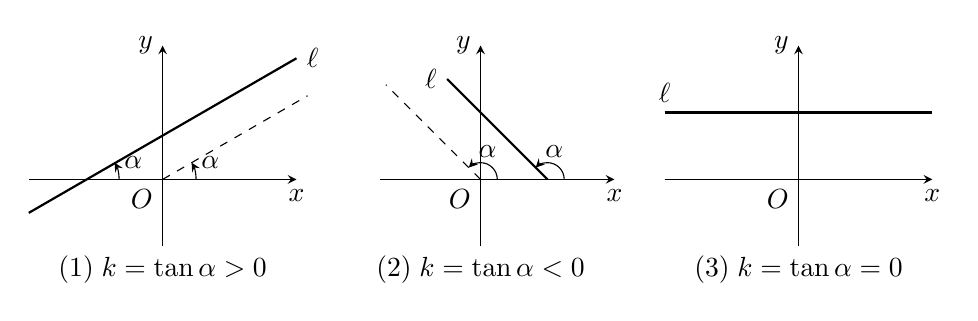
\begin{tikzpicture}[>=stealth, scale=.85]
\begin{scope}
\draw[->](-2,0)--(2,0)node[below]{$x$};
\draw[->](0,-1)node[below]{$(1)\; k=\tan\alpha>0$}--(0,2)node[left]{$y$};
\draw[thick](-2,-.5)--(2,1.81)node[right]{$\ell$};
\draw[dashed](0,0)--(30:2.5);
\draw[->](.5,0) arc (0:30:.5)node[right]{$\alpha$};
\draw[->](-.65,0) arc (0:30:.5)node[right]{$\alpha$};

\node[below left]{$O$};


\end{scope}    
\begin{scope}[xshift=4.75cm]
    \draw[->](-1.5,0)--(2,0)node[below]{$x$};
\draw[->](0,-1)node[below]{$(2)\; k=\tan\alpha<0$}--(0,2)node[left]{$y$};
\draw[thick](1,0)--(-.5,1.5)node[left]{$\ell$};
\draw[dashed](0,0)--(135:2);
\draw[->](.25,0) arc (0:135:.25)node[above right]{$\alpha$};
\draw[->](1.25,0) arc (0:135:.25)node[above right]{$\alpha$};

\node[below left]{$O$};

\end{scope}   
\begin{scope}[xshift=9.5cm]
    \draw[->](-2,0)--(2,0)node[below]{$x$};
\draw[->](0,-1)node[below]{$(3)\; k=\tan\alpha=0$}--(0,2)node[left]{$y$};
\draw[thick](-2,1)node[above]{$\ell$}--(2,1);
\node[below left]{$O$};

\end{scope}   
\end{tikzpicture}
    \caption{}
\end{figure}

因为一条直线只有一个方向，所以当平面直角坐标系选定以后，每一条直线能且只能与一个倾斜角相对应，反之亦
然. 因此，给出了倾斜角就给出了直线的方向.

倾斜角$\alpha$是一个几何对象. 为了用代数方法研究直线，我们再引进倾斜角的代数形式——斜率.

当$\alpha \ne 90^{\circ}$日时，$\alpha$ 的正切值称为直线$\ell$的斜率，记为$k$；

当$\alpha =90^{\circ}$时，也就是$\ell$垂直于$x$轴时，直线$\ell$没有斜率，即
\begin{equation}
\begin{split}
   k= \tan\alpha &\qquad (\alpha\ne 90^{\circ})\\
   k\text{不存在}&\qquad (\alpha= 90^{\circ})
\end{split} \tag{1}
\end{equation}

直线的斜率刻画了直线对于$x$轴的倾斜程度，它是描述直线方向的主要概念，因而将对直线的研究起重要的作用.

\begin{thm}
{思考题}
“在坐标平面上，每一条直线能且只能与一个斜率相对应，反之亦然”. 这句话是不正确的，应如何改正？    
\end{thm}

在坐标平面上，如果已知两个点$P_1(x_1,y_1)$、$P_2(x_2,y_2)$，那么过$P_1$、$P_2$的直线$\ell$就是确定的. 现在研究怎样用这两个点的坐标来表示$\ell$的斜率$k$. 由于$k$是$\alpha$ 的函数，$\alpha$被点$P_1$、$P_2$的位置决定，因此应从具体分析$P_1$、$P_2$的各种相对位置入手解决这个问题（图2.2）.

\begin{figure}[htp]
    \centering
\begin{tikzpicture}[>=stealth]
\begin{scope}
    \draw[->](-1,0)--(3,0)node[below]{$x$};
    \draw[->](0,-1)node[below]{$(1)$}--(0,2)node[left]{$y$};
\node[below left]{$O$};
\draw[thick](-1,1)--node[below]{$\ell_1$}(3,1);
\tkzDefPoints{.5/1/P_1, 2/1/P_2}
\tkzDrawPoints(P_1,P_2)
\tkzLabelPoints[above](P_1,P_2)
  \end{scope}
\begin{scope} [xshift=6.5cm, yshift=-.5cm]
    \draw[->](-1.5,0)--(2.5,0)node[below]{$x$};
    \draw[->](0,-.5)node[below]{$(2)$}--(0,2.5)node[left]{$y$};
\node[below left]{$O$};
\draw[domain=-1.25:1.75, thick, smooth]plot(\x,\x+.8)node[right]{$\ell_2$};
\draw[->](-.8+.35,0) arc (0:45:.35)node[right]{$\alpha$};
\tkzDefPoints{0.2/1/P_1, 1.5/2.3/P_2, 1.5/1/Q}
\tkzDrawPoints(P_1,P_2,Q)
\tkzLabelPoints[above left](P_2)
\tkzLabelPoints[above](P_1)
\tkzLabelPoints[above right](Q)
\draw[dashed](1.5,0)node[below]{$M_2$}--(1.5,2.3);
\draw[dashed](.2,1)--(1.75,1);
\end{scope}
\begin{scope}[yshift=-5cm]
    \draw[->](-1,0)--(2.5,0)node[below]{$x$};
    \draw[->](0,-1)node[below]{$(3)$}--(0,3)node[left]{$y$};
\node[below left]{$O$};
\draw[thick](1,0)--node[right]{$\ell_3$}(1,2.5);
\tkzDefPoints{1/.5/P_2, 1/1.75/P_1}
\tkzDrawPoints(P_1,P_2)
\tkzLabelPoints[right](P_1,P_2)
\end{scope}
\begin{scope}[xshift=6.5cm, yshift=-5cm]
    \draw[->](-1,0)--(3.5,0)node[below]{$x$};
    \draw[->](0,-1)node[below]{$(4)$}--(0,3)node[left]{$y$};
\node[below left]{$O$};
\draw[domain=-.5:2.5, thick]plot(\x, -\x+2)node[below]{$\ell_4$};
\draw[->](2+.25,0) arc (0:135:.25)node[above right]{$\alpha$};
\tkzDefPoints{.5/1.5/P_1, 1.5/.5/P_2, .5/.5/Q}
\tkzDrawPoints(P_1,P_2,Q)
\tkzLabelPoints[above right](P_1,P_2)
\tkzLabelPoints[below right](Q)
\draw[dashed](.5,0)node[below]{$M_1$}--(.5,1.5);
\draw[dashed](0,.5)--(1.5,.5);
\end{scope}
\end{tikzpicture}
    \caption{}
\end{figure}

对于$\ell_1:$ $\because\quad y_1= y_2,\; \ell_1\parallel x$轴，\qquad $\therefore \quad k=0$

对于$\ell_2:$ 过$P_1$作$P_1Q\bot y$轴，过$P_2$作$P_2M_2\bot x$轴，交
$P_{1}Q$ 于$Q$, 则$Q$ 的坐标是($x_2,y_1)$, 且$\alpha=\angle QP_1P_2$,
$$\tan \alpha=\frac{|QP_{2}|}{|P_{1}Q|}=\frac{y_{2}-y_{1}}{x_{2}-x_{1}}$$
若$P_1$, $P_2$的位置互换，则有
$$\tan \alpha=\frac{|QP_{1}|}{|P_{2}Q|}=\frac{y_{1}-y_{2}}{x_{1}-x_{2}}=\frac{y_{2}-y_{1}}{x_{2}-x_{1}}$$

对于$\ell_3:\; x_1=x_2$, $\ell_3\bot x$ 轴，$k$ 不存在；


对于$\ell_4:$ 过$P_1$作$P_1M_1\bot x$轴，作$P_2Q\bot y$ 轴 交 $P_1M_1$于
$Q$,
则 
\[\begin{split}
    \tan\alpha &=\tan(180^{\circ}-\angle QP_{2}P_{1})=-\tan \angle QP_{2}P_{1}\\
    &=-\frac{|P_{1}Q|}{|QP_{2}|}=-\frac{y_{1}-y_{2}}{x_{2}-x_{1}}=\frac{y_{2}-y_{1}}{x_{2}-x_{1}}
\end{split}\]
若$P_1$, $P_2$的位置互换，则有
$$\tan \alpha=-\frac{|P_{2}Q|}{|QP_{1}|}=-\frac{y_{2}-y_{1}}{x_{1}-x_{2}}=\frac{y_{2}-y_{1}}{x_{2}-x_{1}}$$

回 过 头 来 , 对 于 $\ell_{1}$, $k= 0$, 因为 $y_1=y_2$, $x_1\neq x_2$, 所以也
可以写成 $k=\frac{y_2-y_1}{x_2-x_1}$的形式。这样，我们就得到了
\begin{equation}
    \begin{split}
    k=\frac{y_2-y_1}{x_2-x_1} &\qquad \text{当}x_1\ne x_2\\
    k\text{不存在} &\qquad \text{当}x_1= x_2
    \end{split}\tag{2}
\end{equation}
公式(2)直接用$\ell$上两个点的坐标表示出了直线的斜率. 从而为用坐标法研究直线提供了方便.

\begin{thm}
  {思考题}
若直线$\ell$不与$x$轴垂直，并且$\ell$上有三个点：$P_1(x_1,y_1)$、$P_2(x_2,y_2)$、$P_3(x_3,y_3)$. 用$P_1$、$P_2$的坐标算出的$k$值与用$P_1$、$P_3$或$P_2$、$P_3$的坐标算出的$k'$值相同吗？为什么？  
\end{thm}

\begin{example}
    如图2.3，直线$\ell_1$的倾斜角$\alpha_1=30^{\circ}$，直线$\ell_2\bot\ell_1$，求$\ell_1$、$\ell_2$的斜率.
\end{example}

\begin{solution}
$\ell_1$的斜率 $k_1=\tan\alpha_1=\tan30^{\circ}=\frac{\sqrt{3}}{3}$

$\because\quad \ell_2\bot\ell_1$，

$\therefore\quad \ell_2$的倾斜角 $\alpha_2=\alpha_1+90^{\circ}=30^{\circ}+90^{\circ}=120^{\circ}$

$\ell_2$的斜率 $k_2=\tan\alpha_2=\tan120^{\circ}=-\tan 60^{\circ}=-\sqrt{3}$
\end{solution}

\noindent
\begin{minipage}{.45\textwidth}
    \centering
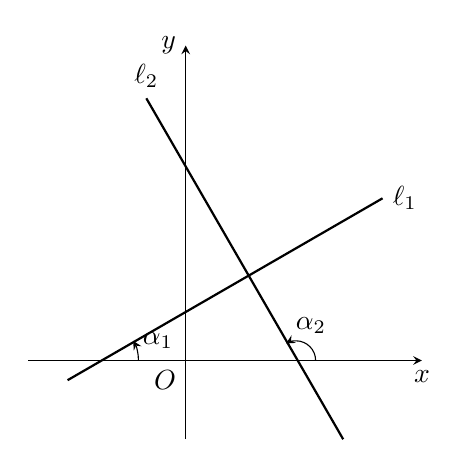
\begin{tikzpicture}[>=stealth]
    \draw[->](-2,0)--(3,0)node[below]{$x$};
    \draw[->](0,-1)--(0,4)node[left]{$y$};
\node[below left]{$O$};

\draw[thick](-1.5,-.25)--(2.5, 1.81+.25)node[right]{$\ell_1$};
\draw[->](-.6,0) arc (0:30:.5)node[right]{$\alpha_1$};
\draw[thick](2,-1)--(-.5, 2.5*1.732-1)node[above]{$\ell_2$};
\draw[->](1.9-.25,0) arc (0:120:.25)node[above right]{$\alpha_2$};

\end{tikzpicture}
\captionof{figure}{}
\end{minipage}
\hfill
\begin{minipage}{.45\textwidth}
    \centering
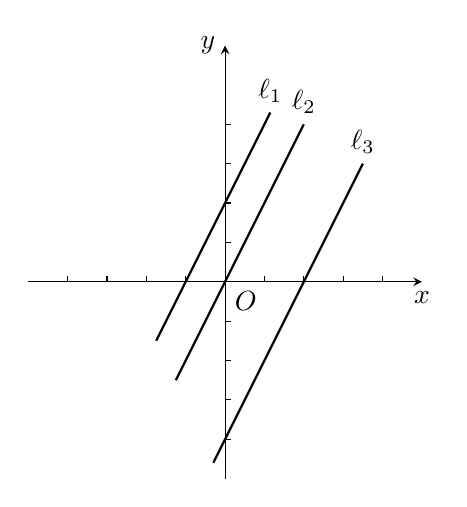
\begin{tikzpicture}[>=stealth, scale=.5]
    \draw[->](-5,0)--(5,0)node[below]{$x$};
    \draw[->](0,-5)--(0,6)node[left]{$y$};
\node[below right]{$O$};
\draw[domain=-1.75:1.15, thick]plot(\x, 2*\x+2)node[above]{$\ell_1$};
\draw[domain=-1.25:2, thick]plot(\x, 2*\x)node[above]{$\ell_2$};
\draw[domain=-.3:3.5, thick]plot(\x, 2*\x-4)node[above]{$\ell_3$};
\foreach \x in {-4,-3,...,4}
{
    \draw(\x,0)--(\x,.15);
    \draw(0,\x)--(.15,\x);
}
\end{tikzpicture} 
\captionof{figure}{}
\end{minipage}

\begin{example}
    求经过$A(-2,0)$、$B(-5,3)$两点的直线的斜率与倾斜角．
\end{example}

\begin{solution}
    由公式(2)，得
\[k=\frac{y_2-y_1}{x_2-x_1}=\frac{3-0}{-5-(-2)}=-1\]
再由公式(1)，得 $-1=\tan\alpha$.

$\because\quad 0\le \alpha<180^{\circ},\qquad \therefore\quad \alpha =135^{\circ}$.

$\therefore\quad$这条直线的斜率是$-1$，倾斜角是$135^{\circ}$．
\end{solution}

最后，再引进直线的纵截距和横截距的概念.

在坐标平面上，对于不平行于$y$轴的直线$\ell$，它与$y$轴交点的纵坐标称为它的\textbf{纵截距}.

如图2.4中的直线$\ell_1$、$\ell_2$、$\ell_3$的纵截距分别是2、0、$-4$．若$\ell\parallel y$轴，它的纵截距没有意义（图2.2(3)）．

同时，对于不平行$x$轴的直线$\ell$，它与$x$轴交点的横坐标称为它的\textbf{横截距}.
如图2.4中的直线$\ell_1$、$\ell_2$、$\ell_3$的横截距分别是$-1$、0、2．若$\ell\parallel x$轴，它的横截距也没有意义［图2.2(1)］．

直线的斜率和截距是在坐标系中刻画直线位置的两个重要参数，应结合图形掌握它们的几何意义.

\begin{thm}
    {思考题} 斜率和截距具有什么特点时直线一定通过II、III、IV象限？I、IV、III象限？
\end{thm}

\begin{ex}
\begin{enumerate}
    \item 填空
\begin{enumerate}[(1)]
    \item 斜率$k$的取值范围是\blank
    \item 当$k>0$时，直线$\ell$一定通过\blank 象限;
    \item 当$k<0$时，直线$\ell$一定通过\blank 象限；
    \item 当$k=0$时，直线$\ell$或通过\blank 象限，或通过\blank 象限，或者\blank; \blank;
    \item 当$k$不存在时，直线$\ell$或通过\blank，或\blank, 或者\blank.
\end{enumerate}

    \item 已知直线的倾角为$\alpha$，求它的斜率
\begin{multicols}{2}
\begin{enumerate}[(1)]
\item $\alpha =0^{\circ}$;
\item $0^{\circ}<\alpha <90^{\circ}$;
\item $\alpha =90^{\circ}$;
\item $90^{\circ}<\alpha <180^{\circ}$.
\end{enumerate}    
\end{multicols}
    \item 求经过下列两点的直线的斜率和倾斜角：
\begin{multicols}{2}
\begin{enumerate}[(1)]
\item $C(-1,\sqrt{3})$ 与 $D(0,0)$
\item $A(3,-8)$ 与 $B(-2,6)$
\item $E(\sqrt{3},-\sqrt{2})$ 与 $F(-\sqrt{2},\sqrt{3})$
\item $G(-2,5)$ 与 $H(-2,-3)$  
\end{enumerate}    
\end{multicols}
\end{enumerate}
\end{ex}

\section{直线方程的几种形式}
确定一条直线需要两个条件，本节将就坐标平面上两个条件的不同给法，根据1.5节的理论分别求出直线$\ell$的不同形式的方程.

\begin{thm}{情况1}
已知直线$\ell$过点$P_0(x_0,y_0)$且斜率是$k$，求直线$\ell$的方程.
\end{thm}

\noindent
\begin{minipage}{.55\textwidth}
\CTEXindent
如图2.5，设$\ell$上异于$P_0$的动点为$P(x,y)$，点$P$运动的规律是过$P_0$、$P$的直线的斜率始终是$k$，即
\[\frac{y-y_0}{x-x_0}=k\quad (x\ne x_0)\]

化简，得
\begin{equation}
    y-y_0=k(x-x_0) \tag{1}
\end{equation}
\end{minipage}
\hfill
\begin{minipage}{.4\textwidth}
\centering
\begin{tikzpicture}[>=stealth]
\draw[->](-2,0)--(3,0)node[below]{$x$};
\draw[->](0,-1)--(0,2.5)node[left]{$y$};
\draw[thick](-1.5, -.2)--(2.5,1.8)node[above]{$\ell$};
\node[below left]{$O$};
\tkzDefPoints{.5/.8/P_0, 2/1.55/P}
\tkzDrawPoints(P_0,P)
\node at (P_0)[below right]{$P_0(x_0,y_0)$};
\node at (P)[below right]{$P(x,y)$};

\end{tikzpicture}
\captionof{figure}{}
\end{minipage}

\begin{proof}
由(1)式的推导，知道，凡是$\ell$上的点其坐标都满足方程(1). 以下证明：(1)的任一个解对应的点都在$\ell$上.

设$\begin{cases}
    x=x_1\\y=y_1
\end{cases}$
是(1)的任一解，即
\begin{equation}
    y_1-y_0=k(x_1-x_0)\tag{$1'$}
\end{equation}

分两种可能：
\begin{enumerate}[(i)]
\item 当$x_1=x_0$时，由($1'$)知$y_1=y_0$，由此，$P_1(x_1,y_1)$与$P_0(x_0,y_0)$重合，

$\therefore\quad P_1(x_1,y_1)$在$\ell$上；
\item 当$x_1\ne x_0$时，由($1'$)得，
\[\frac{y_1-y_0}{x_1-x_0}=k\]
这说明过$P_0$、$P_1$的直线的斜率也是$k$，

$\therefore\quad P_1(x_1,y_1)$在$\ell$上.
\end{enumerate}
\end{proof}

根据曲线与方程的定义. 直线$\ell$的方程是(1).

方程(1)是由直线$\ell$上的一个点和$\ell$的斜率确定的，称为直线方程的\textbf{点斜式}.

当直线$\ell$过点$P_0(x_0,y_0)$，且垂直$y$轴时（图2.6），倾斜角$\alpha=0$, $k=\tan\alpha=0$，由(1)得$\ell$的方程为
\[y-y_0=0(x-x_0)\]
即
\begin{equation}
    y=y_0 \tag{2}
\end{equation}

\noindent
\begin{minipage}{.45\textwidth}
\centering
\begin{tikzpicture}[>=stealth]
    \draw[->](-1,0)--(3.5,0)node[below]{$x$};
\draw[->](0,-1)--(0,3)node[left]{$y$};
\node[below left]{$O$};
\draw[thick](-1,2)--(3,2);
\draw[fill](1.5,2)node[below]{$P_0(x_0,y_0)$} circle(1.5pt);
\tkzDefPoints{0/3/A, 0/2/B, 1/2/C}
\tkzMarkRightAngle(A,B,C)
\end{tikzpicture}
\captionof{figure}{}
\end{minipage}\hfill
\begin{minipage}{.45\textwidth}
    \centering
\begin{tikzpicture}[>=stealth]
    \draw[->](-1,0)--(3.5,0)node[below]{$x$};
    \draw[->](0,-1)--(0,3)node[left]{$y$};
\node[below left]{$O$};

\draw[thick](1.5,-1)--(1.5,2.5);
\draw[fill](1.5,2)node[right]{$P_0(x_0,y_0)$} circle(1.5pt);
\tkzDefPoints{1.5/3/A, 1.5/0/B, 2/0/C}
\tkzMarkRightAngle(A,B,C)

\end{tikzpicture}
\captionof{figure}{}

\end{minipage}

当直线$\ell$过$P_0(x_0,y_0)$，且垂直于$x$轴时（图2.7），倾斜角$\alpha=\frac{\pi}{2}$，$k$不存在，$\ell$的方程不能用(1)表示. 但$\ell$上任一点的横坐标都是，这时，直线的方程是：
\begin{equation}
    x=x_0 \tag{3}
\end{equation}


\begin{thm}
  {情况2} 已知直线$\ell$的斜率是$k$，纵截距是$b$，求$\ell$的方程.  
\end{thm}

此时$\ell$过$(0,b)$点，且斜率为$k$．由公式(1)得
\[y-b=k(x-0)\]
即
\begin{equation}
    y=kx+b \tag{4}
\end{equation}

方程(4)称为直线方程的\textbf{斜截式}.

\begin{thm}
  {情况3} 已知直线$\ell$通过两点$P_1(x_1,y_1)$、$P_2(x_2,y_2)$，求$\ell$的方程.  
\end{thm}

应考虑横坐标$x_1$与$x_2$的关系：
\begin{enumerate}[(1)]
\item 当$x_1=x_2$时，$\ell\bot x$轴，$\ell$的方程是
\[x=x_1\]
\item 当$x_1\ne x_2$时，可转化成点斜式处理. 此时$\ell$的斜率，所以$\ell$的方程可写成
\begin{equation}
y-y_1=\frac{y_2-y_1}{x_2-x_1}(x-x_1)\quad (x_1\ne x_2) \tag{5}    
\end{equation}

方程(5)称为直线方程的\textbf{两点式}.
\end{enumerate}

当$y_2\ne y_1$时，方程(5)还可以写成
\begin{equation}
    \frac{y-y_1}{y_2-y_1}=\frac{x-x_1}{x_2-x_1}\qquad (x_1\ne x_2,\; y_1\ne y_2) \tag{5}
\end{equation}

\begin{thm}
    {情况4} 已知直线$\ell$的纵截距、横截距分别是$b$、$a$（其中$a\ne 0$, $b\ne 0$），求$\ell$的方程（图2.8）．
\end{thm}

\noindent
\begin{minipage}{.55\textwidth}
    \CTEXindent
这种情况可转化成两点式解决. 事实上$\ell$过$P_1(a,0)$、$P_2(0,b)$，代入(5)，得
\[y-0=\frac{b-0}{0-a}(x-a)\]
化简，得
\begin{equation}
    \frac{x}{a}+\frac{y}{b}=1  \tag{6}
\end{equation}    
\end{minipage}
\hfill
\begin{minipage}{.4\textwidth}
\centering
\begin{tikzpicture}[>=stealth]
    \draw[->](-2,0)--(2.5,0)node[below]{$x$};
    \draw[->](0,-1)--(0,2.5)node[left]{$y$};
\node[below left]{$O$};
\tkzDefPoints{-1.5/0/A, 0/1/B}
\tkzDrawLine[add = .2 and 1.3](A,B)
\node at (A)[below]{$a$};
\node at (B)[right]{$b$};
\end{tikzpicture}
\captionof{figure}{}
\end{minipage}


方程(6)称为直线方程的\textbf{截距式}.

到此为止，我们学过了四种形式的方程，它们都表示直线，它们是：
\begin{align}
y-y_0&=k(x-x_0)  \tag{1}\\
y&=kx+b \tag{2}\\
\frac{y-y_1}{y_2-y_1}&=\frac{x-x_1}{x_2-x_1}\quad (x_1\ne x_2,\; y_1\ne y_2)\tag{3}\\
\frac{x}{a}+\frac{y}{b}&=1\quad (a\ne0,\; b\ne 0)\tag{4}
\end{align}

应该知道，不是平面上的所有直线都能写成上述这些形式的方程. 平行于$y$轴的直线不能写成(1)(2)(3)(4)这四种形式，平行于$x$轴的直线不能写成(4)的形式.

上面得到了直线方程的四种特殊形式. 这些方程从代数上看都是关于$x$、$y$的一次方程. 这一事实启迪我们思考：
\begin{enumerate}[(i)]
\item $xOy$平面上的任一条直线，其方程是否都是关于$x$、$y$的一次方程？
\item 关于$x$、$y$的一次方程$Ax+By+C=0$是否都表示$xOy$平面上的一条直线？
\end{enumerate}


这两个问题是直线与一次方程的关系问题，现在分析如下：
\begin{enumerate}[(i)]
    \item $xOy$平面上的所有直线，根据倾斜角$\alpha$是否等于$90^{\circ}$，可以分作两类：

    当$\alpha\ne 90^{\circ}$时，直线的斜率记为$k$，其方程总可以写成$y=kx+b$，
它是关于的一次方程.

当$\alpha=90^{\circ}$时，其方程总可以写成$x=x_0$，即
\[x+0y-x_0=0\]
这个方程仍可以看做关于$x$、$y$的一次方程.

所以，$xOy$平面上的任一直线，其方程都是关于$x$、$y$的一次方程.
\item 要回答关于$x$、$y$的一次方程$Ax+By+C=0$是否都表示直线，讨论如下：

当$B\ne 0$时，方程$Ax+By+C=0$可化成
\[y=-\frac{A}{B}x-\frac{C}{B}\]
这就是直线的斜截式方程，其中$k=-\frac{A}{B}$, $b=-\frac{C}{B}$；

当$B=0$时，则有$A\ne 0$，$Ax+By+C=0$可以写成
\[x=-\frac{C}{A}\]
它表示与$y$轴平行的直线.

所以，关于$x$、$y$的任一个一次方程$Ax+By+C=0$都表示一条直线.
\end{enumerate}

这样，就得到了
\begin{thm}
{定理}
\begin{enumerate}[(i)]
\item $xOy$平面上的任意一条直线，其方程都是关于$x$、$y$的一次方程；
\item 任意一个关于$x$、$y$的一次方程$Ax+By+C=0$（$A$、$B$不同时为零），都表示$xOy$平面上的一条直线.    
\end{enumerate} 
\end{thm}

这个定理很重要，它是上述直线方程的特殊形式在理论上的概括，它揭示了坐标平面上的直线与关于$x$、$y$的一次方程的联系，根据这种联系，研究直线的几何问题就可以和研究一次方程的代数问题互化了.

我们把方程
\begin{equation}
    Ax+By+C=0 \tag{7}
\end{equation}
（其中$A$、$B$不全为零）叫做直线方程的\textbf{一般式}.

对各种形式的直线方程，应注意每个方程适用的条件，并能根据需要灵活地选择直线方程的某种形式进行解题.

\begin{example}
直线$\ell$的方程是$\sqrt{3}x+3y+6=0$\hfill (1)

求$\ell$的斜率、倾斜角和纵截距。
\end{example}

\begin{analyze}
    欲求$k$和纵截距$b$, 须把(1)变成斜截式.
\end{analyze}

\begin{solution}
    由(1)得
\begin{equation}
    y=-\frac{\sqrt{3}}3x-2 \tag{2}
\end{equation}

$\therefore\quad k= - \frac {\sqrt {3}}3$，倾斜角$\alpha=\pi-\arctan\frac{\sqrt{3}}{3}=\frac{5}{6}\pi$, 
纵截距$b=-2$.
\end{solution}

\begin{example}
    直线$\ell$的方程是$\sqrt3x+3y+6=0$\hfill (1)

求$\ell$的横截距和纵截距。
\end{example}

\begin{analyze}
    欲求双截距$a$ 和$b$, 可以采用两种方法：
\end{analyze}

\begin{solution}
\textbf{解法1：}把(1)变成截距式
\[\begin{split}
    \sqrt{3}x+3y&=-6\\
    \frac{\sqrt{3}}{-6}x+\frac{3}{-6}y&=1\\
\frac{x}{-2\sqrt{3}}+\frac{y}{-2}&=1
\end{split}\]
$\therefore\quad a= - 2\sqrt {3},\quad b=-2$.    

\textbf{解法 2：} 用求交点的方法来解。

在(1)中令$y=0$, 得$\sqrt{3} x=-6,\quad  x=-2 \sqrt{3}$,

$\therefore a= - 2\sqrt {3}$ ;    

在(1)中令$x=0$, 得$3y=-6,\quad  y=-2 \sqrt{3}$,

$\therefore b= - 2$.    
\end{solution}

\begin{example}
直线$\ell$的横截距是$-3$，斜率是$-2$，求$\ell$的一般式．
\end{example}

\begin{analyze}
    因为已知斜率和横截距，所以，可写出点斜式方程，再化成一般式.
\end{analyze}

\begin{solution}
$\because\quad \ell$过$(-3,0)$，$k=-2$

$\therefore\quad\ell$的方程是$y=-2(x+3)$. 
即$2x+y+6=0$.
\end{solution}

\begin{thm}
    {思考题} 从一般式入手，能解此题吗？试试看.
\end{thm}

\begin{ex}
\begin{enumerate}
    \item 填空：
\begin{enumerate}[(1)]
\item 经过点$(-2,-3)$，且斜率为$-1$的直线方程是\blank ;
\item 经过点$(-1,-5)$，且倾斜角为$\frac{5\pi}{6}$的直线方程是\blank ;
\item 经过点$(-1,-4)$，且垂直$y$轴的直线方程是\blank ;
\item 经过点$(2,-3)$，且垂直$x$轴的直线方程是\blank ;
\item 斜率为$-2$，纵截距为$-4$的直线方程是\blank；
\item 倾斜角为$\frac{\pi}{3}$，纵截距为$-2$的直线方程是\blank .
\end{enumerate}

    \item 直线$\ell$的方程是$ax+by+c=0$，当系数$a$、$b$、$c$满足什么条件时：
\begin{enumerate}[(1)]
\begin{multicols}{2}
    \item $\ell\bot x$轴;
    \item $\ell$与$x$轴重合；
    \item $\ell$过原点；
    \item $\ell$与两轴都相交；
    \item $\ell$与$x$正半轴相交；    
\end{multicols}
    \item $\ell$的倾斜角为$\frac{\pi}{3}$，且纵截距为2；
    \item $\ell$与坐标轴围成等腰三角形．
\end{enumerate}
\end{enumerate}
\end{ex}

\section*{习题一}
\begin{center}
    \bfseries A
\end{center}

\begin{enumerate}
    \item 若$a$、$b$、$c$是两两不等的实数，求经过下列两点的直线的倾斜角：
\begin{multicols}{2}
\begin{enumerate}[(1)]
\item $A(a,c)$与$B(b,c)$
\item $C(a,b)$与$D(a,c)$
\item $P(b,b+c)$与$Q(a,c+a)$
\end{enumerate}
\end{multicols}

    \item 直线$\ell$的方程是$2x+y-2\sqrt{6}=0$，求其横截距和纵截距.
    \item 已知直线$\ell$的方程是$x-2y+6=0$. 求$\ell$的斜率、倾斜角、横纵截距，并画图.
\end{enumerate}

\begin{center}
    \bfseries B
\end{center}

\begin{enumerate}\setcounter{enumi}{3}
    \item 已知三点$A$、$B$、$C$，若直线$AB$、$AC$的斜率相同，证明这\textbf{三点共线}.
\item     证明：由方程
    \[ax+by+c=0, \quad ax-by+c=0,\quad b\ne 0\]
    确定的两条直线关于$x$轴对称.
\item 证明：直线$ax+by+c=0,\quad (a,b,c\ne 0)$
    和坐标轴围成的三角形的面积为$S=\frac{c^2}{2|ab|}$.
\end{enumerate}

\section{两条直线所成的角}

\noindent
\begin{minipage}{.55\textwidth}
\CTEXindent 
两条直线相交构成四个角，它们是两对对顶角. 为了区别它们，先引入$\ell_1$到$\ell_2$的角的概念．图2.9中的$\theta_{1-2}$表示$\ell_1$绕交点，逆时针第一次转到$\ell_2$形成的角，称为$\ell_1$到$\ell_2$的角；$\theta_{2-1}$表示$\ell_2$绕交点逆时针第一次转到$\ell_1$形成的角，称为$\ell_2$到$\ell_1$的角．

根据上述定义，不难得出：
\end{minipage}
\hfill
\begin{minipage}{.35\textwidth}
\centering
\begin{tikzpicture}[>=stealth, scale=1.3]
\tkzDefPoint(150:1.5){A}
\tkzDefPoint(-30:1.5){B}
\tkzDefPoint(35:1.5){A'}
\tkzDefPoint(35-180:1.5){B'}
\tkzDefPoint(0,0){O}
\draw[thick](A)--(B)node[below]{$\ell_2$};
\draw[thick](B')--(A')node[above]{$\ell_1$};
\tkzMarkAngles[mark=none, ->, size=.4cm](A',O,A)
\tkzMarkAngles[mark=none, ->, size=.3cm](B,O,A')
\tkzLabelAngle[pos=.8](B,O,A'){$\theta_{2-1}$}
\tkzLabelAngle[pos=.7](A',O,A){$\theta_{1-2}$}


\end{tikzpicture}
\captionof{figure}{}
\end{minipage}


\[0<\theta_{1-2}<\pi,\quad 0<\theta_{2-1}<\pi,\quad \theta_{1-2}+\theta_{2-1}=\pi\]

在坐标平面上，$\theta_{1-2}$或$\theta_{2-1}$能否用两条直线的倾斜角表示呢？

先看特殊情况：当至少有一条直线垂直于坐标轴时（图2.10），到角极易算出，请读者试试看．

\begin{figure}[htp]
    \centering
\begin{tikzpicture}[>=stealth]
\begin{scope}
        \draw[->](-2,0)--(3,0)node[below]{$x$};
        \draw[->](0,-1)--(0,4)node[left]{$y$};
        \node[below left]{$O$};
    \draw(1.5,-.75)--(1.5,3.5)node[above]{$\ell_1$};
    
    \tkzDefPoints{0/1/A, 1.5/2.5/B}
    \tkzDrawLine[add=1 and .7](A,B)    
    \draw[->](-.5,0) arc (0:45:.5)node[right]{$\alpha_2$};
    \draw[->](1.5,2.25) arc (-90:45:.25)node[below right]{$\theta_{1-2}$};
    \draw[->](1.5+.4,2.5+.4) arc (45:90:.4*1.414)node[above right]{$\theta_{2-1}$};
    \node at (1.5+1.25,2.5+1.25){$\ell_2$};
    \node at (.5,-1){(1)};
\end{scope}
\begin{scope}[xshift=6cm]
    \draw[->](-1,0)--(4,0)node[below]{$x$};
    \draw[->](0,-1)--(0,4)node[left]{$y$};
    \node[below left]{$O$};
\draw(-1,2)--(3.5,2)node[right]{$\ell_1$};
\node at (1.5,-1){(2)};

\tkzDefPoints{1/2/A, 2/0/B}
\tkzDrawLine[add=.7 and .6](A,B)    
\draw[->](2.5,0) arc (0:116.6:.5)node[above right]{$\alpha_2$};
\draw[->](1.5,2) arc (0:116.6:.5)node[above right]{$\theta_{1-2}$};
\draw[<-](1.6,2) arc (0:-63.4:.6)node[right]{$\theta_{2-1}$};
\node at (0,3.65)[right]{$\ell_2$};
\end{scope}
\end{tikzpicture}
    \caption{}
\end{figure}



现在研究一般情况：已知图（2.11）
\begin{itemize}
    \item $\ell_1:\; y=k_1x+b_1$，倾斜角为$\alpha_1$;
    \item $\ell_2:\; y=k_2x+b_2$，倾斜角为$\alpha_2$.
\end{itemize}

\begin{figure}[htp]
    \centering
\begin{tikzpicture}[>=stealth]
\begin{scope}
    \draw[->](-2,0)--(3,0)node[below]{$x$};
    \draw[->](0,-1)--(0,3)node[left]{$y$};
    \node[below left]{$O$};
\tkzDefPoints{-1/0/A, 2/0/B, 1/2/C, 4/0/B'}
\tkzDrawLine[add=.3 and .4](A,C)  
\tkzDrawLine[add=.3 and .4](B,C)  
\node at (1,-1){(1)};
\tkzMarkAngles[mark=none, size=.5cm, ->](B,A,C B',B,C)
\tkzLabelAngle[pos=.8](B,A,C){$\alpha_1$}
\tkzLabelAngle[pos=.8](B',B,C){$\alpha_2$}
\node (D) at (.5,3){$\ell_2$};
\node (D') at (1.85,3){$\ell_1$};
\tkzMarkAngles[mark=none, size=.4cm, ->](D',C,D)
\tkzLabelAngle[pos=.6](D',C,D){$\theta_{1-2}$}

\end{scope}
\begin{scope}[xshift=6cm]
    \draw[->](-1,0)--(4,0)node[below]{$x$};
    \draw[->](0,-1)--(0,3)node[left]{$y$};
    \node[below left]{$O$};
    \tkzDefPoints{.5/0/A, 3/0/B, 2/1.5/C, 4/0/B'}
    \tkzDrawLine[add=.5 and .6](A,C)  
    \tkzDrawLine[add=.5 and .6](B,C)   
    \node at (1.5,-1){(2)};
    \tkzMarkAngles[mark=none, size=.5cm, ->](B,A,C B',B,C)
    \tkzMarkAngles[mark=none, size=.4cm, ->](C,B,A)
    \tkzLabelAngle[pos=.8](B,A,C){$\alpha_2$}
    \tkzLabelAngle[pos=.8](B',B,C){$\alpha_1$}
    \tkzLabelAngle[pos=.7](C,B,A){$\beta$}
    \node (D) at (3.1,2.65){$\ell_2$};
    \node (D') at (1.5,2.65){$\ell_1$};
    \tkzMarkAngles[mark=none, size=.4cm, ->](B,C,D)
    \tkzLabelAngle[pos=.8](B,C,D){$\theta_{1-2}$}

\end{scope}
\end{tikzpicture}
    \caption{}
\end{figure}


容易看出，$$\theta_{1-2}=\alpha_2-\alpha_1$$
或
\begin{equation}
    \theta_{1-2}=\alpha_2+\beta =\alpha_2+(\pi-\alpha_1)=\pi+(\alpha_2-\alpha_1)\tag{1}
\end{equation}

我们知道，直线的倾斜角和斜率有直接的关系.那么，这里得到的$\theta_{1-2}$能否用$\ell_1$、$\ell_2$的斜率$k_1$、$k_2$表示呢？为此，只要对(1)两边取正切即可：
\begin{equation}
\tan\theta_{1-2}=\frac{\tan\alpha_2-\tan\alpha_1}{1+\tan\alpha_2\tan\alpha_1}=\frac{k_2-k_1}{1+k_2k_1}\quad (1+k_1k_2\ne 0) \tag{2}
\end{equation}

公式(2)称为\textbf{到角公式}．对它应注意：
\begin{enumerate}[(i)]
    \item $\theta_{1-2}$的几何意义；
    \item 公式的结构特征；
    \item 当$\theta_{1-2}$, $\alpha_1$, $\alpha_2$都不等于$\frac{\pi}{2}$时才能使用这个公式.
\end{enumerate}

两个到角$\theta_{1-2}$与$\theta_{2-1}$中，较小的一个更加常用，称为两条直线\textbf{所成的角}（简称\textbf{夹角}）.显然夹角的取值范围是$\left(0,\frac{\pi}{2}\right]$. 若要求夹角$\theta$，由(2)可得
\begin{equation}
    \tan\theta =\left|\frac{k_2-k_1}{1+k_2k_+1}\right|
\end{equation}

\begin{example}
    求直线$\ell_1:\; 2x+y-2=0$和$\ell_2:\; 3x-y+2=0$的夹角.
\end{example}


\begin{solution}
    $\ell_1,\ell_2$的斜率分别是$k_1=-2$, $k_2=3$, 由夹角公式(3)得
\[\tan\theta=\left|\frac{3-(-2)}{1+3\cdot(-2)}\right|=1,\qquad \theta=45^{\circ}\]
$\therefore \quad \ell_1,\ell_2$的夹角为$45^{\circ}$.
\end{solution}


\begin{example}
    已知：$\ell_1:\; x-y-5=0$ 和$\ell_2:\; ax+y=0$, 且$\theta_{1-2}=75^{\circ}$, 求$a$.
\end{example}

\begin{solution}
    $\ell_1$、$\ell_2$的斜率是$k_1=1$, $k_2=-a$. $\theta_{1-2}=75^\circ$. 由公式
$\tan\theta_{1-2}=\frac{k_2-k_1}{1+k_2k_1}$，得
    $$\tan 75^{\circ}=\frac{-a-1}{1+1\cdot(-a)}$$

解这个关于$a$的方程（注意$\tan75^{\circ}=2+\sqrt{3}$）得$a=\sqrt{3}$.
\end{solution}


\begin{example}
 过点$P(2,-1)$引直线$\ell'$，使它与直线$\ell:\; 5x-2y+3=0$ 的夹角为$45^{\circ}$. 求 $\ell'$的方程.
\end{example}

\begin{solution}
    只要求出$\ell'$的斜率$k'$就行了. 因为$\ell$的斜率$k=\frac{5}{2}$, 由夹角公式，得
\begin{minipage}{.55\textwidth}
\[\tan45^{\circ}=\left|\frac{k'-k}{1+k'k}\right|=\left|\frac{k'-\frac{5}{2}}{1+\frac{5}{2}k'}\right|\]
即
\[\frac{k'-\frac{5}{2}}{1+\frac{5}{2}k'}=\pm 1 \quad  \Rightarrow \quad \frac{2k'-5}{2+5k'}=\pm 1\]
解得：$k'_1=-\frac{7}{3},\quad k'_2=\frac{3}{7}$. 从而，$\ell'$有两条（图2.12），它们的方程分别是
\[y+1=-\frac{7}{3}(x-2)\quad \text{和}\quad y+1=\frac{3}{7}(x-2)\]
\end{minipage}
\hfill
\begin{minipage}{.4\textwidth}
\centering
\begin{tikzpicture}[>=stealth, scale=.8]
\draw[->](-2.5,0)--(3.5,0)node[above]{$x$};
\draw[->](0,-4)--(0,4)node[left]{$y$};
\node[below left]{$O$};
\draw[domain=-2:.8, smooth, very thick]plot(\x, 2.5*\x+1.5)node[above]{$\ell$};
\tkzDefPoints{.45/2.62/A, -1.62/-2.55/B, 2/-1/P}
\tkzDrawPoints(A,B,P)
\tkzDrawLines[add = .2 and .4](A,P B,P)
\tkzMarkAngles[size=.5, mark=none](B,A,P P,B,A)
\tkzLabelAngle[pos=.85](B,A,P){$\tfrac{\pi}{4}$}
\tkzLabelAngle[pos=.85](P,B,A){$\tfrac{\pi}{4}$}
\node at (P)[right]{$P(2,-1)$};

\node at (3.75,-.4){$\ell'_2$};
\node at (2.75,-2.7){$\ell'_1$};
\end{tikzpicture}
\captionof{figure}{}
\end{minipage}
即：
$\ell'_1:\; 7x+3y-11=0$和$\ell'_2:\; 3x-7y-13=0$.
\end{solution}

\begin{ex}
\begin{enumerate}
    \item 求下列各组直线的夹角.
\begin{enumerate}[(1)]
    \item $\ell_1:\; x-2y-10=0,\qquad   \ell_2:\; 3x-y+2=0$
    \item $\ell_1:\; 3x+4y+6=0,\qquad   \ell_2:\; y-3=0$
    \item $\ell_1:\; x+2=0,\qquad     \ell_2:\; 3x-3y=0$
\end{enumerate}
    \item 已知直线$\ell_1$过原点，且$\ell_1$到$\ell_2:\; y=2x-5$的角是$135^{\circ}$，求: $\ell_1$的方程.
\end{enumerate}
\end{ex}


\section{两条直线平行或垂直的条件}
对于两条存在斜率的直线
\begin{itemize}
    \item $\ell_1$：斜率为$k_1$，倾斜角为$\alpha_1$,
    \item $\ell_2$：斜率为$k_2$，倾斜角为$\alpha_2$.
\end{itemize}

\subsection{平行（或重合）条件}

\noindent
\begin{minipage}{.55\textwidth}
    \CTEXindent
若$\ell_1$与$\ell_2$平行（或重合）（图2.13)
\[\alpha_1=\alpha_2 \quad \Rightarrow\quad k_1=k_2\]

若$k_1=k_2\quad \Rightarrow\quad \alpha_1=\alpha_2$（注意$\alpha$的取值范围是$0\le \alpha<\pi$，且$\alpha\ne \frac{\pi}{2}$)
\[\ell_1\parallel \ell_2\quad \text{或}\quad \ell_1\text{与}\ell_2\text{重合}\]

于是
\end{minipage}
\hfill
\begin{minipage}{.4\textwidth}
\centering
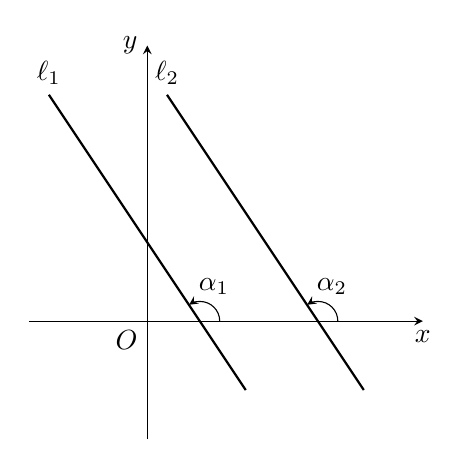
\begin{tikzpicture}[>=stealth]
    \draw[->](-1.5,0)--(3.5,0)node[below]{$x$};
    \draw[->](0,-1.5)--(0,3.5)node[left]{$y$};
    \node[below left]{$O$};
    \draw[domain=1.25:-1.25, thick, smooth]plot(\x, -1.5*\x+1)node[above]{$\ell_1$};
    \draw[domain=1.25:-1.25, thick, smooth]plot(\x+1.5, -1.5*\x+1)node[above]{$\ell_2$};.
    \draw[->](0.67+.25,0)arc (0:123.7:.25)node[above right]{$\alpha_1$};
    \draw[->](0.67+1.75,0)arc (0:123.7:.25)node[above right]{$\alpha_2$};
\end{tikzpicture}
\captionof{figure}{}
\end{minipage}

\begin{equation}
    \ell_1\parallel \ell_2 \text{（或$\ell_1$ 与$\ell_2$重合）} \Longleftrightarrow k_1=k_2  \tag{1}
\end{equation}

对于(1)要注意它的前提是$\ell_1,\ell_2$都存在斜率.


\subsection{垂直条件}
当$\ell_1\bot\ell_2$时，到角$\theta_{1-2}=\frac{\pi}{2}$，$\tan\theta_{1-2}$不存在，我们把到角公式写成
\begin{equation}
    \cot \theta_{1-2}=\frac{1+k_2k_1}{k_2-k_1} \tag{*}
\end{equation}


若$\ell_2\bot \ell_2$, 到角$\theta_{1-2}=\frac{\pi}{2}\quad \Rightarrow\quad \cot\theta_{1-2}=0$
\[\begin{cases}
    1+k_2k_1=0\\
    k_2-k_1\ne 0
\end{cases}\Rightarrow\quad k_1k_2=-1\]

若$k_1k_2=-1$
\[\begin{cases}
    1+k_2k_1=0\\
    k_2-k_1\ne 0
\end{cases}\Rightarrow\quad \cot\theta_{1-2}=0\quad \Rightarrow\quad    \theta_{1-2}=\frac{\pi}{2}\quad \Rightarrow\quad \ell_1\bot\ell_2\]

$\therefore\quad \ell_1\bot\ell_2 \Longleftrightarrow k_1k_2=-1$ \hfill(2)

注意：(2)成立的前提也是$\ell_1,\ell_2$都存在斜率.

(1)与(2)也可用$\ell_1,\ell_2$的方程的系数表示：

设$\ell_1:\; a_1x+b_1y+c_1=0$, $\ell_2:\; a_2x+b_2y+c_2=0$.

把$k_1=-\frac{a_1}{b_2}$, $k_2=-\frac{a_2}{b_2}$代入(1)，得
\begin{equation}
    k_1=k_2\Longleftrightarrow a_1b_2-a_2b_1=0\quad \text{（平行或重合）} \tag{3}
\end{equation}
代入(2)，得
\begin{align}
    k_1k_2=-1 &\Longleftrightarrow \left(-\frac{a_1}{b_1}\right)\left(-\frac{a_2}{b_2}\right)=-1 \nonumber\\
    &\Longleftrightarrow a_1a_2+b_1b_2=0 \quad \text{（垂直）} \tag{4}
\end{align} 

经验证，知道：
\begin{thm}{结论1}
    若$\ell_1$或$\ell_2$的斜率不存在，(3)和(4)仍然成立. 即：
\[\begin{split}
    \ell_1\parallel \ell_2 \text{（或$\ell_1$与$\ell_2$重合）} &\Longleftrightarrow a_1b_2-a_2b_1=0\\
    \ell_1\bot \ell_2  &\Longleftrightarrow a_1a_2+b_1b_2=0\\
\end{split}\]
\end{thm}


\begin{thm}{结论2}
    若$\ell$的方程是$ax+by+c=0$,
\begin{enumerate}[(1)]
\item 与$\ell$平行的直线的一般形式是：
\begin{equation}
    ax+by+m=0\quad \text{（$m$是参数）} \tag{5}
\end{equation}

\item 与$\ell$垂直的直线的一般形式是：
\begin{equation}
    bx-ay+m=0\quad \text{（$m$是参数）} \tag{6}
\end{equation}
\end{enumerate}
\end{thm}

这两条结论在应用上很重要，证明留给读者.





\begin{example}
已知直线$\ell_1:\; 2x-4y+7=0$，$\ell_2:\; x-2y+5=0$，
    求证：$\ell_1\parallel \ell_2$
\end{example}

\begin{analyze}
    只要证出$k_1=k_2$且其纵截距不相等即可.
\end{analyze}

\begin{solution}
    把$\ell_1,\ell_2$的方程写成斜截式：
\[\ell_1:\; y=\frac{1}{2}x+\frac{7}{4},\qquad \ell_2:\; y=\frac{1}{2}x+\frac{5}{2}\]
则$\ell_1$的斜率$k_1=\frac12$, 纵截距$b_1=\frac74$； $\ell_2$的斜率$k_2=\frac12$, 纵截距$b_2=\frac52$

$\therefore\quad k_1=k_2,\; b_1\ne b_2\quad \Rightarrow\quad \ell_1\parallel \ell_2$
\end{solution}


\begin{example}
    求过点$(2,1)$且与直线$\ell_1:\; 2x+y-10=0$垂直的直线$\ell_2$的方程.
\end{example}

\begin{analyze}
    利用$\ell_1\bot\ell_2\Longleftrightarrow k_1k_2=-1$可求得$\ell_2$的斜率$k_2$，再用点斜式可写出$\ell_2$ 的方程. 也可用本节结论(6)去作.
\end{analyze}

\begin{solution}
\textbf{解法1：}容易得出，$\ell_1$的斜率$k_1=-2$，由$\ell_1\bot\ell_2\Longleftrightarrow k_1k_2=-1$，可得
\[(-2)\cdot k_2=-1\Longleftrightarrow k_2=\frac{1}{2}\]
又因$\ell_2$过$(2,1)$点，知其方程是
\[y-1=\frac{1}{2}(x-2)\quad \Rightarrow\quad x-2y=0\]

\textbf{解法2：}由$\ell_1\bot \ell_2$，且$\ell_1$的方程是$2x+y-10=0$，知$\ell_2$的方程应具有形式
\begin{equation}
    x-2y+m=0  \tag{*}
\end{equation}

又$\because\quad \ell_2$过点$(2,1)$，

$\therefore\quad $点$(2,1)$的坐标应适合(*)，即
\[2-2\x1+m=0\quad \Rightarrow\quad m=0\]

$\therefore\quad \ell_2$的方程是$x-2y=0$.
\end{solution}

\begin{example}
    用坐标法解：
正方形$ABCD$中，$E$是$BC$边的中点，$F$是$AB$延长线上的一点，问$F$在什么位置时，$AE\bot CF$成立？
\end{example}

\begin{analyze}
如图2.14建立坐标系，设$F(x,0)$，利用$AE\bot CF\Longleftrightarrow k_{AE}\cdot k_{CF}=-1$，建立以$x$为“元”的方程，求$x$即可.
\end{analyze}

\begin{solution}
如图2.14建立坐标系，则有$B(1,0)$、$C(1,1)$、$D(0,1)$、$E\left(1,\frac{1}{2}\right)$. 设$F$的坐标为$(x,0)$. 显然，直线$AE$、$CF$的斜率都存在：
\[  k_{AE}=\frac{\frac{1}{2}-0}{1-0}=\frac{1}{2},\quad
    k_{CF}=\frac{1-0}{1-x}=\frac{1}{1-x}
 \]
利用$AE\bot CF\Longleftrightarrow k_{AE}\cdot k_{CF}=-1$，得
\[\frac{1}{2}\cdot \frac{1}{1-x}=-1\quad \Rightarrow\quad x=\frac{3}{2}\]
$\therefore\quad $当$BF=\frac{1}{2}AB$时就有$AE\bot CF$.
\end{solution}


\noindent
\begin{minipage}{.45\textwidth}
\centering
\begin{tikzpicture}[>=stealth]
\draw[->](-1,0)--(4,0)node[below]{$x$};
\draw[->](0,-1)--(0,4)node[left]{$y$};
\node[below left]{$A(O)$};
\tkzDefPoints{0/2/D, 3/0/F, 2/0/B, 2/2/C, 2/1/E,0/0/A}
\draw(D)--(C)--(B);
\draw(F)--(C);
\node at (B)[below, text width=1cm, align=center]{$B$\\$(1,0)$};
\node at (F)[below, text width=1cm, align=center]{$F$\\$(x,0)$};
\node at (C)[right]{$C(1,1)$};
\node at (D)[above right]{$D(0,1)$};
\tkzInterLL(A,E)(C,F) \tkzGetPoint{G}
\draw(A)--(G);
\node at (E)[left]{$E$};
\tkzMarkRightAngle[size=.2](A,G,F);
\end{tikzpicture}
\captionof{figure}{}
\end{minipage}
\hfill
\begin{minipage}{.45\textwidth}
\centering
\begin{tikzpicture}[>=stealth, scale=.5]
\tkzDefPoints{3/-4/A, 1/3/B, -4/-2/C}
\tkzDrawPolygon(A,B,C)
\tkzLabelPoints[left](C)
\tkzLabelPoints[above](B)
\node at (A)[right]{$A(3,-4)$};
\tkzDefPointBy[projection=onto B--A](C) \tkzGetPoint{E}
\tkzDefPointBy[projection=onto C--A](B) \tkzGetPoint{F}
\tkzDrawLines[add=0 and .3](C,E B,F)
\tkzMarkRightAngles[size=.3](C,E,A B,F,A)
\node at (3.5,0.5){$\ell_2$};
\node at (-1.5,-5){$\ell_1$};

\end{tikzpicture}
\captionof{figure}{}
\end{minipage}


\begin{example}
在$\triangle ABC$中，已知$A(3,-4)$和分别过点$B$、$C$的两条高所在的直线方程是$\ell_1:\; 7x-2y-1=0$与$\ell_2:\; 2x-7y-6=0$，求三边所在的直线的方程.
\end{example}

\begin{analyze}
    做解析几何题，画出图，直观形象，便于数形结合.但是，有时画图不易（如这里要在坐标系中画出$\triangle ABC$就不容易）.这时，可以画示意图代替在坐标系中画图.
\end{analyze}

\begin{solution}
    画出示意图（图2.15).

$\because\quad $直线$AC\bot \ell_1$, $\ell_1$的方程是：$7x-2y-1=0$,

$\therefore\quad AC$的方程具有形式$2x+7y+m=0$.

又$\because\quad AC$过$A(3,-4)$，可定出$m=22$,

$\therefore\quad AC$的方程是$2x+7y+22=0$

同理，$AB$的方程可求出，为$7x+2y-13=0$. 

点$B(x,y)$可由$\begin{cases}
    7x-2y-1=0\\ 7x+2y-13=0
\end{cases}$求出，为$B(1,3)$；

点$C(x,y)$可由$\begin{cases}
    2x-7y-6=0\\ 2x+7y+22=0
\end{cases}$求出，为$C(-4,-2)$.

$\therefore\quad BC$的方程是$y-3=\frac{3-(-2)}{1-(-4)}(x-1)$，即
\[x-y+2=0\]
\end{solution}

\begin{ex}
\begin{enumerate}
    \item 判断下列各对直线是否平行、垂直或重合：
\begin{enumerate}[(1)]
\item $y=3x+4$ 与 $2y-6x+1=0$;
\item $y=x$ 与 $3x+3y-10=0$;
\item $3x+4y-5=0$ 与 $6x-8y-7=0$;
\item $\sqrt{3}x-y-1=0$ 与 $\sqrt{3}x+3y+6=0$;
\item $\sqrt{2}x+\sqrt{3}y=\sqrt{6}$ 与 $2x+\sqrt{6}y-2\sqrt{3}=0$.
\end{enumerate}

    \item 求过点$A(2,3)$，且分别适合下列条件的直线方程：
\begin{enumerate}[(1)]
    \item 平行于直线$2x+y-7=0$;
    \item 垂直于直线$3x-2y+5=0$.
\end{enumerate}
    \item 已知两直线$\ell_1,\ell_2$，其中$\ell_1$没有斜率. $\ell_1$与$\ell_2$什么时候
    （1）平行；（2）垂直？其逆命题成立吗？
\end{enumerate}
\end{ex}

\section{两条直线的交点}
设两条直线为
\[\begin{split}
 \ell_1:&\; a_1x+b_1y+c_1=0\\
\ell_2:&\; a_2x+b_2y+c_2=0   
\end{split}\]

根据1.4节的推论，求$\ell_1$、$\ell_2$的交点的问题等价于解方程组
\[\begin{cases}
    a_1x+b_1y+c_1=0 &(1)\\
    a_2x+b_2y+c_2=0 &(2)
\end{cases}\]
的问题.

\begin{itemize}
    \item 若方程组有唯一解$(x_0,y_0)$，则$\ell_1$、$\ell_2$相交于$(x_0,y_0)$;
    \item 若方程组无解，则$\ell_1\parallel \ell_2$；
    \item 若方程组有无穷多解，则$\ell_1$重合于$\ell_2$．
\end{itemize}

设$a_1$、$a_2$、$b_1$、$b_2$全不为零，解这个方程组：

$(1)\times b_2$，得
\begin{equation}
    a_1b_2x+b_1b_2y+b_2c_1=0 \tag{3}
\end{equation}
$(2)\times b_1$，得
\begin{equation}
    a_2b_1x+b_1b_2y+b_1c_2=0 \tag{4}
\end{equation}
$(3)-(4)$得
\[(a_1b_2-a_2b_1)x+(b_2c_1-b_1c_2)=0\]
即
\begin{equation}
    (a_1b_2-a_2b_1)x=b_1c_2-b_2c_1 \tag{5}
\end{equation}

\begin{enumerate}
    \item 当$a_1b_2-a_2b_1\neq0$时，(5)有唯一解，从而可求出方程
组的唯一解：
\[\begin{cases}
    x=\frac{b_1c_2-b_2c_1}{a_1b_2-a_2b_1}\\
    y=\frac{a_2c_1-a_1c_2}{a_1b_2-a_2b_1}
\end{cases}\]
这时，$\ell_1,\ell_2$相交，上面$x$和$y$ 的值就是交点的坐标. 这是因为$\ell_1,\ell_2$的斜率分别是$-\frac {a_1}{b_1}$和$-\frac{a_2}{b_2}$, 由$a_1b_2-a_2b_1\neq0$可知$\frac{a_1}{b_1}\neq\frac{a_2}{b_2}$, 也就是$-\frac {a_1}{b_1}\neq-\frac{a_2}{b_2}$, 这说明$\ell_1,\ell_2$的斜率不等，所以$\ell_1,\ell_2$必相交于一点.

例如，两条直线
\[\begin{split}
    2x-3y+4&=0\\
    3x+y-5&=0
\end{split}\]
由于$\frac23\neq\frac3{-1}$（斜率不等），也就是$\frac23\neq\frac{-3}1$（$x$、$y$项的对应
系数不成比例），这两个方程组成的方程组就有唯一解，这个
解是
$$\begin{cases}x=1\\y=2\end{cases}$$
也就是两条直线相交于点$(1,2)$.

\item 当$a_1b_2-a_2b_1=0$时，
\begin{enumerate}[(i)]
    \item  若 $b_1c_2-b_2c_1\neq0$，(5)无解，从而方程组无解. 事实上，这时$c_1,c_2$不可能全为零，不妨设$c_2\neq0$, 有$\frac {a_1}{a_2}=\frac{b_1}{b_2}\neq\frac{c_1}{c_2}$, 也就是$\frac{a_1}{b_1}=\frac{a_2}{b_2}$, 且$\frac {c_1}{b_1}\neq\frac{c_2}{b_2}$, 所以，$\ell_1,\ell_2$的斜率相等：$-\frac{a_1}{b_1}=-\frac{a_2}{b_2}$, 
而纵截距不等，$\frac{c_1}{b_1}\neq\frac{c_2}{b_2}$, 此时，$\ell_1\parallel \ell_2$.

例如，两条直线
\[\begin{split}
    3x-y+2&=0\\6x-2y-5&=0
\end{split}\]
由于$\frac{3}{6}=\frac{-1}{-2}\ne\frac{2}{-5}$，所以方程组无解，也就是两直线平行.
\item 若$b_1c_2-b_2c_1=0$，(5)有无穷多解，从而方程组也有无穷多解. 事实上，此时$c_1$、$c_2$ 或全为零或全不为零（当$c_1,c_2$ 全不为零时，$\frac{a_1}{a_2}=\frac{b_1}{b_2}=\frac{c_1}{c_2}$），两个方程是同解方程，所以它们有无穷多解，也就是两条直线重合.

例如，两条直线
\[\begin{split}
    3x-y+2&=0\\
    6x-2y+4&=0
\end{split}\]
由于$\frac{3}{6}=\frac{-1}{-2}=\frac{2}{4}$, 两个方程是同解方程，方程组有无穷多
解，因而两直线重合.
\end{enumerate}
\end{enumerate}

对于$a_1,a_2,b_1,b_2$有等于零的情况，方程组比较简单，
同学们可自己进行讨论.








\begin{example}
    根据下列每组直线的方程判断两条直线的位置关系（相交？平行？重合？），若相交，求出交点坐标：
\begin{enumerate}[(1)]
\item $\ell_1:\; 3x-2y-6=0;\qquad \ell_2:\; 9x+4y+7=0$
\item $\ell_1:\; 3x-2y-6=0;\qquad \ell_2:\; 4y-6x-3=0$
\end{enumerate}
\end{example}
 
\begin{solution}
\begin{enumerate}[(1)]
    \item 解方程组$\begin{cases}
        3x-2y=6\\ 9x+4y=-7
    \end{cases}$
得
$\begin{cases}
    x=\frac{1}{3}\\y=-\frac{5}{2}
\end{cases}$

$\ell_1,\ell_2$相交于$\left(\frac{1}{3},-\frac{5}{2}\right)$
\item 解方程组
$\begin{cases}
    3x-2y=6\\ -6x+4y=3
\end{cases}$

$\because\quad \frac{3}{-6}=\frac{-2}{4}\ne \frac{6}{3}$

$\therefore\quad \ell_1,\ell_2$平行.
\end{enumerate}
\end{solution}


\begin{example}
    已知两直线
\[\begin{split}
  \ell_1:&\; x+my+6=0\\
  \ell_2:&\; (m-2)x+3y+2m=0 
\end{split}\]
求当$m$为何值时，$\ell_1$与$\ell_2$：（i）相交；（ii）平行；（iii）重合.
\end{example}

\begin{solution}
解方程组$\begin{cases}
    x+my=-6\\ (m-2)x+3y=-2m
\end{cases}$
\[\begin{split}
  a_1b_2-a_2b_1&=1\x3-(m-2)m=3-m^2+2m\\
b_1c_2-b_2c_1&=m(-2m)-3(-6)=-2m^2+18  
\end{split}\]

令$a_1b_2-a_2b_1=0$，即$-m^2+2m+3=0$，解得$m=3$, $m=-1$.

令$b_1c_2-b_2c_1=0$，即$-2m^2+18=0$，解得$m=\pm 3$.

\begin{enumerate}[(i)]
\item 当$m\ne 3$，且$m\ne -1$时，$a_1b_2-a_2b_1\ne 0$，方程组有唯一解，$\ell_1$与$\ell_2$相交；
\item 当$m=-1$时，$a_1b_2-a_2b_1=0$, $b_1c_2-b_2c_1\ne 0$，方程组无解，$\ell_1$与$\ell_2$平行；
\item 当$m=3$时，$a_1b_2-a_2b_1=0$，$b_1c_2-b_2c_1=0$，方程组有无穷多解，$\ell_1$与$\ell_2$重合． 
\end{enumerate}
\end{solution}

\begin{ex}
\begin{enumerate}
    \item 求下列各对直线的交点，并画图：
\begin{enumerate}[(1)]
    \item $\ell_1:\; 2x-y=1,\qquad \ell_2:\; 3x+2y=19$
    \item $\ell_1:\; x=2,\qquad \ell_2:\; 3x+2y-12=0$
\end{enumerate}

    \item 判定下列各对直线的位置关系.若相交，求出交点坐标：
\begin{enumerate}[(1)]
\item $4x-3y-8=0$与$3x-y=0$;
\item $2x-6y+4=0$与$y=\frac{x}{3}+\frac{2}{3}$;
\item $(\sqrt{2}-1)x+y=3$与$x+(\sqrt{2}+1)y=2$;
\item $2x-3y=5$与$4x-6y=10$.
\end{enumerate}

    \item 当$a$，$b$取何值时，直线$ax-2y-1=0$与$6x-4y-b=0$.
\begin{multicols}{3}
\begin{enumerate}[(1)]
    \item 相交；
    \item 平行；
    \item 重合．
\end{enumerate}
\end{multicols}
    \item 已知直线满足下列条件，求直线的方程：
\begin{enumerate}[(1)]
\item 过直线$3x-y+4=0$与$x+y-4=0$的交点，且斜率为$-2$；
\item 过直线$x-2y+3=0$与$x+2y-9=0$的交点和原点.
\end{enumerate}

\end{enumerate}
\end{ex}

\section*{习题二}
\begin{center}
    \bfseries A
\end{center}

\begin{enumerate}
    \item  已知直线$\ell:\; y=x+5$. 求过点$A(5,2)$且与直线$\ell$的夹角为$45^{\circ}$的直线的方程．
    \item 已知三角形三边所在的直线方程分别是：
\[\begin{split}
    AB:&\; x-y-3=0\\
    BC:&\; x-3y+3=0\\
    AC:&\; 2x+y+5=0\\
\end{split}\]
    试求三个内角（用反三角函数表示）.
    \item 已知两点$A(2,2)$、$B(5,-2)$．在横轴上求一点$P$，使$\angle APB$为直角．你还能把此题推广吗？
    \item 直线$(3a+2)x+(1-4a)y+8=0$和$(5a-2)x+(a+4)y-7=0$互相垂直. 试求$a$的值. 提示：利用本节结论(4).
    \item 求证：对于$\alpha\in [0,\pi]$，直线
    $x\sin\alpha+y\cos\alpha+1=0$
    总与直线
    $x\cos\alpha-y\sin\alpha+2=0$
    垂直.
    \item 求证：直线$x+2y-5=0$, $2x+4y+5=0$, $2x-y=0$, $7x-11y-35=0$围成一个直角梯形.
    \item 直线$ax+2y+8=0$, $4x+3y=10$和$2x-y=10$相交于一点，求$a$值.
    \item 不解方程组，判断下列两方程的直线的位置关系：
\begin{multicols}{2}
\begin{enumerate}[(1)]
    \item $\begin{cases}
        3x-y=4\\ 2x+3y=5
    \end{cases} $
    \item $\begin{cases}
        3x+2y=6\\ 6x+4y=12
    \end{cases} $
    \item $\begin{cases}
        x-3y=-4\\3x-9y=10
    \end{cases} $
    \item $\begin{cases}
        12x-6y=-6 \\ 8x-4y=4
    \end{cases} $
\end{enumerate}
\end{multicols}
\end{enumerate}

\begin{center}
    \bfseries B
\end{center}

\begin{enumerate}\setcounter{enumi}{8}
    \item  直线上依次有四个点$A$、$B$、$C$、$D$，且$AB=BC=CD$. $P$为以$BC$为直径的半圈上的任一点（$P$与$B$、$C$都不重合）. 记$\angle APB=\alpha$, $\angle CPD=\beta$，求证$\tan\alpha\cdot \tan\beta$为定值.
    \item 已知两条直线
\[\begin{split}
     \ell_1:&\; (3+m)x+4y=5-3m\\
    \ell_2:&\; 2x+(5+m)y=8   
\end{split}\]
$m$为何值时，$\ell_1$
    与$\ell_2$：
    （1）相交；（2）平行；（3）重合．
    \item 若$P(a,b)$为第一象限内的一个定点，过点$P$的动直线交$x$、$y$轴的正方向于$M$、$N$. 求证：$\triangle OMN$面积的最小值为$2ab$．
\end{enumerate}

\section*{三、点与直线的位置关系}
点与直线的位置关系可分为两类：一是点在直线上，一是点不在直线上. 对于已知点$A$的坐标，和直线$\ell$的方程时，如何判断点$A$在直线$\ell$上或不在$\ell$上我们已讨论过了. 下面讨论当$A$不在直线$\ell$上时，如何求$A$到直线$\ell$的距离. 以及点$A$关于直线$\ell$的对称点的坐标的求法.

\section{点到直线的距离}
已知一个点$P(x_0,y_0)$和直线$\ell:\; ax+by+c=0$，本节将研究如何求出点$P$到直线$\ell$的距离$d_{P-\ell}$.

我们知道，点$P$到直线$\ell$的距离是点$P$到直线$\ell$的垂线段的长. 欲求$d_{P-\ell}$先从两种特例入手：
\begin{enumerate}
    \item 当直线$\ell$平行坐标轴时（也就是系数$a$，$b$中有一个为零时，图2.16）．

    容易看出，对于图2.16（1），$d_{P-\ell}=|y_0-y_1|$，对于图2.16(2), $d_{P-\ell}=|x_0-x_1|$.

\begin{figure}[htp]
    \centering
\begin{tikzpicture}[>=stealth]
\begin{scope}
\draw[->](-1,0)--(4,0)node[below]{$x$};
\draw[->](0,-2)--(0,3)node[left]{$y$};
\draw(-1,-1)--(3.5,-1)node[right]{$\ell$};
\draw(2,2)node[above]{$P(x_0,y_0)$}--node[right]{$d_{P-\ell}$}(2,-1)node[below]{$Q$};
\node[below left]{$O$};
\node at (2,-2){(1)};
\tkzDefPoints{2/2/P, 2/-1/Q, 3/-1/L}
\tkzMarkRightAngles[size=.2](P,Q,L)
\node at (3,-1)[below]{$y=y_1$};
\tkzDrawPoints(P)

\end{scope}
\begin{scope}[xshift=7cm]
\draw[->](-1,0)--(4,0)node[below]{$x$};
\draw[->](0,-1)--(0,3)node[left]{$y$};
\draw(2,-1)node[below]{$x=x_1$}--(2,2.5)node[above]{$\ell$};
\draw(-1,2)node[above]{$P(x_0,y_0)$}--node[above]{$d_{P-\ell}$}(2,2)node[right]{$Q$};
\node[below left]{$O$};
\node at (2,-2){(2)};
\tkzDefPoints{-1/2/P, 2/2/Q, 2/-1/L}
\tkzMarkRightAngles[size=.2](P,Q,L)
\tkzDrawPoints(P)
    
\end{scope}
\end{tikzpicture}
    \caption{}
\end{figure}


\item 当点$P$落在坐标轴上时（图2.17）．

容易看出，点$A$、$B$的坐标易算出，进而线段$OA$、$OB$、$PA$、$AB$的长可求，利用$\triangle PQA\backsim \triangle AOB$，有
\[\frac{|PQ|}{|PA|}=\frac{|OB|}{|AB|}\quad \Rightarrow\quad d_{P-\ell}=\frac{|PA|\cdot |OB|}{|AB|}\]
\end{enumerate}

现在研究一般情况.

当点$P(x_0,y_0)$不在坐标轴上时，过点$P$作$PM\parallel y$轴，
交$\ell$于点$M$（图2.18）则
仍有$\triangle PQM\backsim \triangle AOB$：
\begin{equation}
    \frac{|PQ|}{|PM|}=\frac{|OB|}{|AB|}\quad \Rightarrow\quad d_{P-\ell}=\frac{|PM|\cdot |OB|}{|AB|}\tag{*}
\end{equation}

我们只要用$a$、$b$、$c$、$x_0$、$y_0$表示$|PM|$, $|OB|$, $|OA|$, 就可表示出$d_{P-\ell}$. 容易求得$M$、$A$、$B$的坐标分别是
\[\left(x_0,\; \frac{-ax_0-c}{b}\right),\quad \left(0,\; -\frac{c}{b}\right),\quad \left(-\frac{c}{a},\; 0\right)\]

\noindent
\begin{minipage}{.47\textwidth}
    \centering
\begin{tikzpicture}[>=stealth]
    \draw[->](-1,0)--(4,0)node[below]{$x$};
    \draw[->](0,-1)--(0,4)node[left]{$y$};
\node[below left]{$O$};
    \tkzDefPoints{0/2/A, 2.5/0/B}
\tkzDrawLines[add=.3 and .3](A,B)
\tkzDefPoints{0/3/P}
\tkzDefPointBy[projection = onto A--B](P) \tkzGetPoint{Q}
\draw(Q)--node[above left]{$d_{P-\ell}$}(P)node[right]{$P(0,y_0)$};
\tkzLabelPoints[right](A)
\tkzLabelPoints[below](B,Q)
\tkzMarkRightAngles[size=.2](P,Q,B)
\node at (3,-.5)[below]{$\ell$};
\end{tikzpicture}    
\captionof{figure}{}
\end{minipage}\hfill
\begin{minipage}{.47\textwidth}
    \centering
\begin{tikzpicture}[>=stealth]
    \draw[->](-1,0)--(4,0)node[below]{$x$};
    \draw[->](0,-1)--(0,4)node[left]{$y$};
\node[below left]{$O$};
\tkzDefPoints{0/2/A, 2.5/0/B, 2/2/P, 2/1/P', 0/0/O}
\tkzDrawLines[add=.3 and .3](A,B)
\tkzDefPointBy[projection = onto A--B](P) \tkzGetPoint{Q}
\tkzLabelPoints[right](A)
\tkzLabelPoints[below](B,Q)
\draw(Q)--(P)node[above]{$P(x_0,y_0)$};
\tkzMarkRightAngles[size=.2](P,Q,B)
\node at (3,-.5)[below]{$\ell$};
\tkzInterLL(P,P')(A,B) \tkzGetPoint{M}
\draw[dashed](P)--(M)node[right]{$M$};
\tkzMarkAngles[size=.3, mark=none](O,A,B P,M,A)

\end{tikzpicture}    
\captionof{figure}{}
\end{minipage}

于是
\[|OA|=\left|-\frac{c}{b}\right|=\left|\frac{c}{b}\right|,\quad |OB|=\left|-\frac{c}{a}\right|=\left|\frac{c}{a}\right| \]
\[\begin{split}
    |AB|&=\sqrt{|OA|^2+|OB|^2}=\sqrt{\frac{c^2}{b^2}+\frac{c^2}{a^2}}=\left|\frac{c}{ab}\right|\sqrt{a^2+b^2}\\
    |PM|&=\left|y_0+\frac{ax_0+c}{b}\right|=\frac{|ax_0+by_0+c|}{|b|}
\end{split}\]
代入(*)式，得
\[d_{P-\ell}=\frac{|ax_0+by_0+c|}{|b|}\cdot \frac{|c|}{|a|}\cdot \frac{|ab|}{|c|\sqrt{a^2+b^2}}\]
即
\begin{equation}
    d_{P-\ell}=\frac{|ax_0+by_0+c|}{\sqrt{a^2+b^2}}
\end{equation}

这就是点$P(x_0,y_0)$到直线$ax+by+c=0$的距离公式.

利用公式(1)以$(0,0)$代替$(x_0,y_0)$得\textbf{原点$O$到直线$\ell$的距离}：
\begin{equation}
    d_{O-\ell}=\frac{|c|}{\sqrt{a^2+b^2}} \tag{2}
\end{equation}

下面我们讨论\textbf{两平行直线$\ell_1,\ell_2$间的距离}.

设$\ell_1:\; ax+by+c_1=0$、$\ell_2:\; ax+by+c_2=0$, 
（两方程的系数仅仅$c_1\ne c_2$）

\begin{enumerate}
    \item 若$\ell_1$、$\ell_2$位于原点的两侧（如图2.19（1）），则
\[d_{\ell_1-\ell_2}=d_1+d_2=\frac{|c_1|}{\sqrt{a^2+b^2}}+\frac{|c_2|}{\sqrt{a^2+b^2}}=\frac{|c_1-c_2|}{\sqrt{a^2+b^2}}\]
（注意：此时$c_1,c_2$符号相反！）

\item 若$\ell_1$、$\ell_2$位于原点的同一侧（如图2.19（2）），则
\[d_{\ell_1-\ell_2}=d_1-d_2=\frac{|c_1|}{\sqrt{a^2+b^2}}-\frac{|c_2|}{\sqrt{a^2+b^2}}=\frac{|c_1-c_2|}{\sqrt{a^2+b^2}}\]
（注意：此时$c_1,c_2$符号相同！）

\begin{figure}[htp]
    \centering
\begin{tikzpicture}[>=stealth]
\begin{scope}
    \draw[->](-2,0)--(3,0)node[below]{$x$};
    \draw[->](0,-2)node[below]{(1)}--(0,2.5)node[left]{$y$};
  \node[below right]{$O$};
\draw[domain=-1:2, thick]plot(\x, -\x+1)node[right]{$\ell_1$};
\draw[domain=-2:1, thick]plot(\x, -\x-1)node[right]{$\ell_2$};
\draw[very thick](0.5,.5)--node[above left]{$d_1$}(0,0)--node[above left]{$d_2$}(-.5,-.5);
\tkzDefPoints{.5/.5/A1, -.5/-.5/A2, 1/0/B1, 0/-1/B2}
\tkzMarkRightAngles[size=.15](A1,A2,B2  A2,A1,B1)
\draw[decorate, decoration={brace, amplitude=5pt}](O)--(A1);
\draw[decorate, decoration={brace, amplitude=5pt}](A2)--(O);



\end{scope}
\begin{scope}[xshift=8cm]
    \draw[->](-4,0)--(1,0)node[below]{$x$};
    \draw[->](0,-2)--(0,2.5)node[left]{$y$};
  \node[below right]{$O$};
  \draw[domain=-1:-3.5, thick]plot(\x, \x+3)node[below]{$\ell_1$};
  \draw[domain=.2:-2.3, thick]plot(\x, \x+1)node[below]{$\ell_2$};
  \tkzDefPoints{-.5/.5/A2, -1.5/1.5/A1, 0/0/O}
\draw(A1)--(O);
\draw[decorate, decoration={brace, amplitude=5pt}](O)--node[below left]{$d_2$}(A2);
\draw[decorate, decoration={brace, amplitude=5pt}](A1)--node[above right]{$d_1$}(O);
\node at (-1.5,-2)[below]{(2)};


\end{scope}
\end{tikzpicture}
    \caption{}
\end{figure}

\item 若$\ell_1$、$\ell_2$中有一条通过原点时，即$c_1,c_2$有一个为零，易得
\[d_{\ell_1-\ell_2}=\frac{|c_1|}{\sqrt{a^2+b^2}}\quad \text{或}\quad d_{\ell_1-\ell_2}=\frac{|c_2|}{\sqrt{a^2+b^2}}\]
\end{enumerate}

综合上述三种情况，都有
\begin{equation}
    d_{\ell_1-\ell_2}=\frac{|c_1-c_2|}{\sqrt{a^2+b^2}} \tag{3}
\end{equation}

\begin{example}
\begin{enumerate}[(1)]
    \item 求点$P(3,-3)$到$\ell:\; x=2y+4$的距离；
    \item 原点到直线$y+2=k(x-3)$的距离为2，求此直线的方程.
\end{enumerate}
\end{example}

\begin{solution}
\begin{enumerate}[(1)]
    \item 把$\ell$的方程写成一般式$x-2y-4=0$.
由公式(1)，得
\[d_{P-\ell}=\frac{|ax_0+by_0+c|}{\sqrt{a^2+b^2}}=\frac{1\x 3+(-2)(-3)-4|}{\sqrt{1^2+(-2)^2}}=\sqrt{5}\]
\item 欲求直线的方程，求出$k$就行了．

把直线的方程写成一般式$kx-y-(3k+2)=0$，依题，有
\[d_{0-e}=\frac{|3k+2|}{\sqrt{k^2+1^2}}=2\]
解之，得$k_1=0,\quad k_2=-\frac{12}{5}$.
\begin{itemize}
    \item 当$k_1=0$时，直线方程为$y=-2$；
    \item 当$k_2=-\frac{12}{5}$时，直线方程为$12x+5y-26=0$.
\end{itemize}
\end{enumerate}
\end{solution}

\begin{example}
求两条平行线间的距离，若
$$\ell_1:\; 2x-7y+8=0,\qquad \ell_2:\; 4x-14y-12=0$$
\end{example}   

\begin{solution}
先把$\ell_2$的方程变为$2x-7y-6=0$，
再由公式(3)，得
\[d_{\ell_1-\ell_2}=\frac{|c_1-c_2|}{\sqrt{a^2+b^2}}=\frac{|8-(-6)|}{\sqrt{2^2+7^2}}=\frac{14\sqrt{53}}{53}\]
\end{solution}

\noindent
\begin{minipage}{.5\textwidth}
\begin{example}
已知直线
\[\begin{split}
\ell_1:\; &    x-2y-2=0\\
\ell_2:\; &2x+y-10=0
\end{split}\]
求$\ell_1$、$\ell_2$的交角平分线的方程. 
\end{example}

\begin{analyze}
    作出草图2.20交角平分线为$t_1,t_2$. 由于交角平分线的特征性质是其上任一点到角的两边距离相等. 因此，可归结为点到直线的距离处理.
\end{analyze}
\end{minipage}\hfill
\begin{minipage}{.47\textwidth}
    \centering
\begin{tikzpicture}[>=stealth, scale=.5]
  \draw[->](-2,0)--(8,0)node[below]{$x$};
  \draw[->](0,-4.5)--(0,5.5)node[left]{$y$};
\node[below left]{$O$};
\draw[domain=-1:6.5, thick]plot(\x, 0.5*\x-1)node[right]{$\ell_1$};
\draw[domain=6.55:3, thick]plot(\x, 10-2*\x)node[right]{$\ell_2$};

\draw[domain=2.75:5.5, thick, dashed]plot(\x, 3*\x-12)node[right]{$t_1$};
\draw[domain=7.5:-1, thick, dashed]plot(\x, 2.667-.333*\x)node[left]{$t_2$};

\tkzDefPoints{2/0/A1, 4/1/A2, 2/6/B1, 3/4/B2, 3/-3/P}
\tkzDefPointBy[projection= onto A1--A2](P) \tkzGetPoint{C1}
\tkzDefPointBy[projection= onto B1--B2](P) \tkzGetPoint{C2}
\draw[dashed](C1)--(P)node[below right]{$P(x,y)$}--(C2);
\end{tikzpicture}    
\captionof{figure}{}
\end{minipage}

\begin{solution}
如图2.20设$P(x,y)$为交角平分线上的动点，则
\begin{equation}
    d_{P-\ell_1}=d_{P-\ell_2} \tag{1}    
\end{equation}
即
\[\frac{|x-2y-2|}{\sqrt{1^2+(-2)^2}}=\frac{|2x+y-10|}{\sqrt{2^2+1^2}}\]
化简为$|x-2y-2|=|2x+y-10|$.

由绝对值的定义得
\[x-2y-2=\pm (2x+y-10)\]
即
\begin{equation}
   x+3y-8=0\quad \text{或}\quad 3x-y-12=0 \tag{2}
\end{equation}
\end{solution}

\subsection*{2.6 练习}
\begin{enumerate}
\item 求下列点到直线的距离：
\begin{enumerate}[(1)]
\item $A(-2,3)$与$\ell:\; 3x-4y+3=0$
\item $B(-1,0)$与$\ell:\; \frac{x}{2}-\frac{y}{\sqrt{3}}=1$
\item $C(1,-2)$与$\ell:\; 3x+3y=0$
\item $O(0,0)$与$\ell:\; y=\frac{26}{5}x-3$
\item 原点与$\ell:\; x=3y$    
\item 原点与$\ell:\; x\cos\alpha+y\sin\alpha=4$，其中$\alpha\in[0,2\pi]$.
\end{enumerate}

\item 求平行线$3x-2y-7=0$与$6x-4y=15$间的距离.
\item 三角形三个顶点是$A(7,8)$、$B(10,4)$和$C(2,-4)$，计算它的$BC$边上的高的长.
\end{enumerate}



\section{关于直线的对称点}
在平面几何中已学习过对称的概念.

若直线$\ell$垂直平分线段$AA'$，则点$A'$称为点$A$\textbf{关于直线
$\ell$的对称点}. 类似地若点$M$是线段$AA'$的中点，则点$A'$称为点$A$\textbf{关于点$M$的对称点}.

容易得到：
\begin{itemize}
\item 点$A(x,y)$关于$x$轴的对称点是$A'(x,-y)$;
\item 点$A(x,y)$关于$y$轴的对称点是$A''(-x,y)$;
\item 点$A(x,y)$关于原点$O$的对称点是$P(-x,-y)$;
\item 点$A(x,y)$关于直线$y=x$的对称点是$Q(y,x)$;
\item 点$A(x,y)$关于直线$y=-x$的对称点是$Q'(-y,-x)$.
\end{itemize}

已知点$P(x_0,y_0)$和直线$\ell:\; ax+by+c=0\; (ab\ne 0)$.

若点$P'(x',y')$是点$P$关于$\ell$的对称点（图2.21）本节将研究$x',y'$如何用$x_0,y_0$表示.

分析如下：

$\because\quad $点$P'$与$P$关于$\ell$对称，

$\therefore\quad \ell$垂直平分线段$PP'$. 我们知道：
    \begin{align}
    \ell\bot PP' &\Longleftrightarrow k_{\ell}\cdot k_{PP'}=-1 \tag{$A$}\\
    \ell\text{平分}PP' &\Longleftrightarrow PP'\text{的中点在$\ell$上}\tag{$B$}
    \end{align}
    
    由此，$x',y'$由方程组
    \[\begin{cases}
    \frac{-a}{b}\cdot \frac{y'-y_0}{x-x_0}=-1& (A')\\[1.5ex]
    a\cdot \frac{x'+x_0}{2}+b\cdot \frac{y'+y_0}{2}+c=0&(B')
    \end{cases}\]
    确定. 解这个方程组就可以求出$x'$、$y'$.


\noindent
\begin{minipage}{.45\textwidth}
    \centering
\begin{tikzpicture}[>=stealth]
  \draw[->](-2,0)--(2.5,0)node[below]{$x$};
  \draw[->](0,-1)--(0,4)node[left]{$y$};
\node[below left]{$O$};
\tkzDefPoints{1/0/A, 0/1.5/B}
\tkzDrawLines[add= 1 and .7](B,A)
\tkzDefPoints{.5/3/P}
\tkzDefPointBy[projection= onto A--B](P) \tkzGetPoint{P''}
\tkzDefPointWith[linear, K=2](P,P'') \tkzGetPoint{P'}
\draw[dashed](P)node[right]{$P(x_0,y_0)$}--(P')node[below]{$P'(x',y')$};
\tkzDrawPoints(P,P')
\node at (-1,3)[above]{$\ell$};
\end{tikzpicture}    
\captionof{figure}{}
\end{minipage}\hfill
\begin{minipage}{.5\textwidth}
    \centering
\begin{tikzpicture}[>=stealth, scale=.58]
  \draw[->](-4,0)--(6,0)node[below]{$x$};
  \draw[->](0,-3.5)--(0,5)node[left]{$y$};
\node[below left]{$O$};
\foreach \x in {1,2,3}
{
    \draw(\x,0)--(\x,.1);
    \draw(-.1,-\x)--(0,-\x);
    \draw(-.1,\x)--(0,\x);
    \draw(-\x,0)--(-\x,.1);
}
\tkzDefPoints{-1/3/B, 2/0/N, 4/-2/A', 4/2/A}
\tkzDrawLines[add =0 and .5, very thick](N,B)
\tkzDrawSegments[dashed](A,A' A',N)
\tkzDrawSegments[very thick](A,N)
\node at (A)[above]{$A(4,2)$};
\node at (A')[below]{$A'(4,-2)$};
\node at (B)[below left]{$B(-1,3)$};
\node at (N)[below]{$N$};
\tkzDrawPoints(A,B,A')
\end{tikzpicture}    
\captionof{figure}{}
\end{minipage}


下面以例题的形式研究光线的反射问题.

\begin{example}
    通过点$A(4,2)$的光线，经$x$轴反射后通过点$B(-1,3)$．求入射线和反射线所在直线的方程及反射点．
\end{example}

\begin{analyze}
 解光线反射问题必须把握光线运动的“最短路径原理”，即光线在同一种媒质中前进时必通过最短的路径. 在本题中，光线从点$A$射来，经$x$轴反射（反射点为$N$），通过点$B$而去，则$|AN|+|NB|$应为“最短”（图2.22）．
\end{analyze}

\begin{solution}
    如图2.22，设反射点为$N(x,0)$，则$AN$就是入射线，$NB$
就是反射线.我们利用“最短路径原理”来确定点$N$的坐标.

取$A(4,2)$关于$x$轴的对称点$A'(4,-2)$. 欲使
$|AN|+|NB|$
为最短，从平面几何知道，须使点$N$位于直线$A'B$与$x$轴的交点上，因为直线$A'B$的方程是
\[y+2=\frac{3-(-2)}{-1-4}(x-4)\]
即$y+2=-(x-4)$.

所以，点$N$的坐标$(x,0)$须满足
\[\begin{cases}
    y+2=-(x-4)\\
    y=0   
\end{cases}\]
解之，得$x=2$，故反射点$N(2,0)$.

由此，入射线$AN$所在直线的方程是
\[y-0=\frac{2-0}{4-2}(x-2)\]
即$x-2y-2=0$.

反射线$NB$所在直线的方程就是$A'B$的方程，即$x+y-2=0$.
\end{solution}

\begin{rmk}
此题也可以用光的反射原理“入射角等于反射角”去考虑（留给读者去作）.
\end{rmk}

\begin{example}
     已知$A(3,1)$、$B(-1,3)$和$\ell:\; 2x+4y-5=0$，光线由$A$射来，经过$\ell$反射后再通过$B$，求反射线方程和反射点.
\end{example}

\begin{analyze}
    这个题与例2.18的不同处在于例2.18是光线经由$x$轴反射（即反射点在$x$轴上），而例2.19却以直线$\ell$代替了$x$轴（图2.23）．但是，两个例子的实质是相同的，因此可用相同的方法.
\end{analyze}

\begin{solution}
设$A(3,1)$关于$\ell$的对称点为$A'(x',y')$，则$x'$、$y'$可以从方程组

\noindent
\begin{minipage}{.5\textwidth}\CTEXindent
    \[\begin{cases}
        \frac{y'-1}{x'-3}\cdot \left(-\frac{1}{2}\right)=-1\\[1.5ex]
    2\cdot \frac{x'+3}{2}+4\cdot \frac{y'+1}{2}-5=0
    \end{cases}\]
    解出，为$\begin{cases}
        x'=2\\y'=-1
    \end{cases}\Rightarrow\quad A'(2,-1)$

    欲使$|AN|+|NB|$为最短，须使反射点$N$位于$A'B$与直线$\ell$的交点上. $A'B$的方程（即反射线所在直线的方程）是
    \[y+1=\frac{3-(-1)}{-1-2}(x-2)\]
    即$4x+3y-5=0$.
\end{minipage}\hfill
\begin{minipage}{.47\textwidth}
    \centering
\begin{tikzpicture}[>=stealth, scale=.9]
  \draw[->](-2,0)--(4,0)node[below]{$x$};
  \draw[->](0,-2)--(0,4.5)node[left]{$y$};
\node[below left]{$O$};
\draw[domain=-1.75:3.5, thick]plot(\x, -0.5*\x+1.25);
\tkzDefPoints{-1/3/B, 3/1/A, 1/.75/E, 2/.25/F}
\tkzDefPointBy[projection= onto E--F](A)\tkzGetPoint{A''}
\tkzDefPointWith[linear, K=2](A,A'') \tkzGetPoint{A'}
\tkzInterLL(B,A')(E,F)  \tkzGetPoint{M}
\draw[very thick](B)node[above]{$B(-1,3)$}--(M)--(A)node[above]{$A(3,1)$};
\draw[dashed, thick](M)--(A')node[below]{$A'(x',y')$}--(A);
\tkzDrawPoints(A',A,B)
\foreach \x in {1,2,3}
{
    \draw(\x,0)--(\x,.1);
    \draw(0,\x)--(.1,\x);
}
\node at (-2,2.25){$\ell$};

\end{tikzpicture}    
\captionof{figure}{}
\end{minipage}

反射点$N$的坐标由$\begin{cases}
    2x+4y-5=0\\ 4x+3y-5=0
\end{cases}$
解出，为$N\left(\frac{1}{2},\; 1\right)$.
\end{solution}


从这两个例子可以看出：解光的反射问题的依据是光的最短路径原理或光的反射原理（入射角等于反射角）.反映在数学上，其工具是求点关于直线的对称点的方法.

\subsection*{2.7 练习}
\begin{enumerate}
\item 光线经过点$(2,3)$，在直线$x+y+1=0$上反射，反射线经过点$(1,1)$，求光线的入射线和反射线所在直线的方程及反射点.
\item 光线经过点$P(-2,5)$和点$Q(1,1)$，然后被$x$轴反射，求反射点及反射线所在直线的方程.
\item 光线经点$A(-3,5)$射到直线$3x-4y+4=0$上，反射点为$P$，反射线通过点$B(8,9)$，求证：$|AP|+|PB|=13$.
   \item 在直线$2x+y-5=0$上求一点$P$，使它到$A(-7,1)$和$B(-5,5)$的距离之和为最小．
\end{enumerate}

\section*{习题三}
\begin{center}
    \bfseries A
\end{center}

\begin{enumerate}
    \item 已知直线$\ell:\; y-3=k(x+1)$，点$P(1,-1)$、点$Q(3,1)$.
\begin{enumerate}[(1)]
    \item 若$\ell$到点$P$的距离为2，求$\ell$的方程；
    \item 若$\ell$到点$P$与到点$Q$距离相等，求$k$．
\end{enumerate}
\item \begin{enumerate}[(1)]
\item 求经过原点，并且和$P(2,1)$的距离等于1的直线方程。
\item 求与直线$7x+24y-5=0$平行，并且距离等于3的直线方程.
\item 已知两平行直线$\ell_1:\; ax+by+c_1=0$与$\ell_2:\; ax+by+c_2=0$,

求证：与$\ell_1,\ell_2$距离相等的直线的方程是$ax+by+\frac{c_1+c_2}{2}=0$.
\end{enumerate}

\item 
求下列各对直线的交角平分线的方程：
\begin{enumerate}[(1)]
    \item $x+3y-6=0$与$3x+y+2=0$.
    \item $12x-5y-60=0$与$5x+12y-24=0$.
\end{enumerate}

\item 已知$\triangle ABC$三顶点为$A(2,6)$、$B(7,1)$和$C(-1,-3)$, 求三角形内角$A$的平分线所在的直线方程.
\item 已知点$A(a,5)$到直线$3x-4y=2$的距离为$d$，

问当$a$取何值时：(1)$d=4$; \qquad (2)$d>4$.



\noindent
\begin{minipage}{.47\textwidth}
\item 上面的例题讲的都是一个镜面的反射问题（例2.18以$x$轴作镜面，例2.19以直线$\ell$作镜面）．能否把这个问题推广到有几个镜面的情形呢？如，平面上有两条直线$\ell_1$、$\ell_2$以及点$P$和$Q$. 欲使从点$P$发出的光线依次经$\ell_1$、$\ell_2$反射后通过点$Q$. 试以几何方法找出$\ell_1$上的反射点$M$.


\end{minipage}\hfill
\begin{minipage}{.47\textwidth}
    \centering
\begin{tikzpicture}[>=stealth, scale=1.5]
  \draw(-2,1)node[left]{$\ell_1$}--(1,-.5);
  \draw(-2,-1)node[left]{$\ell_2$}--(1,.5);
\tkzDefPoints{-1.75/.35/P, -1/-.15/Q}
\tkzDrawPoints(P,Q)
\tkzLabelPoints[left](P,Q)


\end{tikzpicture}    
\captionof*{figure}{题6}
\end{minipage}

\item 以$A(4,5)$为顶点，在$ox$轴上找一点$B$，在直线$\ell:\; 2x-y+2=0$上找一点$C$，构成$\triangle ABC$，使$|AB|+|BC|+|CA|$为最小，并求出这个最小值.
\end{enumerate}

\begin{center}
    \bfseries B
\end{center}

\begin{enumerate}\setcounter{enumi}{7}
    \item 设$O(0,0)$、$A(t,0)$、$B\left(t,\frac{1}{t}\right)$是$xy$平面上的三个点（其中$t>0$），$\triangle OAB$的重心$G$到三边$OA$、$AB$、$OB$的距离依次为$p$、$q$、$r$，求证$pqr$的最大值为$\frac{\sqrt{2}}{54}$.
    \item 光线从点$M(5,3)$射出，被直线$\ell:\; x+y-1=0$反射，入射线到直线$\ell$的角为$\beta$. 已知$\tan\beta=2$，求入射线与反射线所在直线的方程.
\end{enumerate}


\section*{四、直线系}

\section{直线系的概念}
我们知道确定一条直线需要两个条件.若只给出一个条件，直线是不能唯一地确定的.实际上，这时，可以得到满
足这个条件的一系列直线。
如，斜率为$\frac{1}{2}$的直线就有无数条（图2.24）．这无数条直线的方程具有共同的形式
\begin{equation}
    y=\frac{1}{2}x+b \tag{1}
\end{equation}
其中$b$为相应直线的纵截距，当$b$取不同的值时，方程(1)表示不同的直线（实际上方程表示的直线与$b$的取值是一一对应
的），我们称它为\textbf{参数}，再如，过点$(3,2)$的直线也有无数条（图2.25），它们的方程却具有共同形式
\begin{equation}
    y-2=k(x-3)\quad \text{或}\quad x=3\tag{2}
\end{equation}
其中$k$为相应直线的斜率，它也是一个参数.

\noindent
\begin{minipage}{.47\textwidth}
    \centering
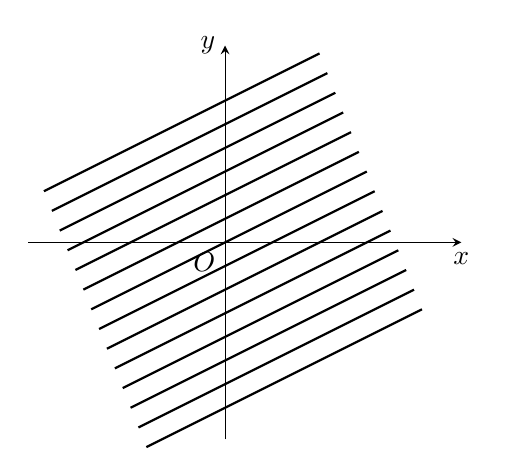
\begin{tikzpicture}[>=stealth]
  \draw[->](-2.5,0)--(3,0)node[below]{$x$};
  \draw[->](0,-2.5)--(0,2.5)node[left]{$y$};
\node[below left]{$O$};
\foreach \y in {0,1,2,...,13}
{
    \draw[domain=-1-\y*.1:2.5-\y*.1, thick]plot(\x, {0.5*\x+\y*0.3-2.1});
}
\end{tikzpicture}    
\captionof{figure}{}
\end{minipage}\hfill
\begin{minipage}{.47\textwidth}
    \centering
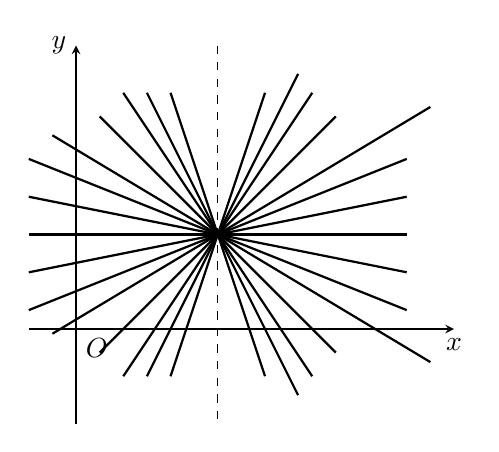
\begin{tikzpicture}[>=stealth, scale=.6]
  \draw[->](-1,0)--(8,0)node[below]{$x$};
  \draw[->](0,-2)--(0,6)node[left]{$y$};
\node[below right]{$O$};

\draw[domain=-1:7, thick]plot(\x, {0*(\x-3)+2});
\draw[domain=-1:7, thick]plot(\x, {0.2*(\x-3)+2});
\draw[domain=-1:7, thick]plot(\x, {0.4*(\x-3)+2});
\draw[domain=-.5:7.5, thick]plot(\x, {0.6*(\x-3)+2});
\draw[domain=.5:5.5, thick]plot(\x, {1*(\x-3)+2});
\draw[domain=1:5, thick]plot(\x, {1.5*(\x-3)+2});
\draw[domain=-1:7, thick]plot(\x, {-0.2*(\x-3)+2});
\draw[domain=-1:7, thick]plot(\x, {-0.4*(\x-3)+2});
\draw[domain=-.5:7.5, thick]plot(\x, {-0.6*(\x-3)+2});
\draw[domain=.5:5.5, thick]plot(\x, {-1*(\x-3)+2});
\draw[domain=1:5, thick]plot(\x, {-1.5*(\x-3)+2});
\draw[domain=1.5:4.7, thick]plot(\x, {-2*(\x-3)+2});
\draw[domain=1.5:4.7, thick]plot(\x, {2*(\x-3)+2});
\draw[domain=2:4, thick]plot(\x, {-3*(\x-3)+2});
\draw[domain=2:4, thick]plot(\x, {3*(\x-3)+2});
\draw[dashed](3,6)--(3,-2);




\end{tikzpicture}    
\captionof{figure}{}
\end{minipage}

一般地，我们把满足一个共同条件的直线的集合（直线的系列）称为一个\textbf{直线系}，把表示直线系的方程叫做\textbf{直线系方程}（它一定含有一个参数）.

很明显，直线系被它的共同条件（请注意，有且只有一个条件）所确定. 因此要研究一个直线系必须紧紧抓住它的共同条件. 此外，还须注意，有时一个直线系需要用两个方程来表示它（如上述过$(3,2)$的直线系）．

为什么要引入直线系的概念呢？我们知道，求一条直线的方程，需要给出两个条件. 当根据这两个条件不便于直接写出直线的方程时，可以先择其一，写出它的直线系方程，再用待定系数法，根据第二个条件确定参数的值，从而求出直线的方程.

\begin{example}
填写满足下列条件的直线系方程：
\begin{enumerate}[(1)]
\item 斜率为$-2$的直线系方程是($y=-2x+b$),
\item 倾角为$\frac{1}{3}\pi$的直线系方程是($y=\sqrt{3}x+b$);
\item 与直线$ax+by+c=0$平行的直线系方程是
($ax+by+m=0$);
\item 与直线$ax+by+c=0$垂直的直线系方程是
($bx-ay+m=0$).
\item 经过点$(-2,-3)$的直线系方程是
[$y+3=k(x+2)$ 与$x=-2$];
\item 双截距的和为4的直线系方程是$\left(\frac{x}{a}+\frac{y}{4-a}=1\right)$.
\end{enumerate}
\end{example}

\begin{example}
     求与$\ell:\; 2x+3y-7=0$垂直且过$P(-1,-3)$的直线$\ell'$的方程.
\end{example}

\begin{solution}
    \textbf{解法1：}可求得$k=\frac{-2}{3}\quad \Rightarrow\quad k'=\frac{3}{2}$
    
    又因为$\ell'$过$P(-1,-3)$，所以$\ell'$的方程是
\[y+3=\frac{3}{2}(x+1)\quad \Rightarrow\quad 3x-2y-3=0\]

\textbf{解法2：}与$\ell$垂直的直线系方程为
\[3x-2y+m=0\]
其中，过$P(-1,-3)$的一条$\ell'$应满足
\[3(-1)-2(-3)+m=0\]
解之$m=-3$，所以$\ell'$的方程是$3x-2y-3=0$.
\end{solution}

\begin{remark}
    解法2体现了用直线系解题的基本思想；先写出满足一个条件（与$\ell$垂直）的所有直线($3x-2y+m=0$)，再根据第二个条件（过$P$点）定出参数的值，从而求出所需的直线方程.
\end{remark}

\begin{example}
    求经过点$(-5,5)$且和原点的距离为1的直线$\ell$的方程．
\end{example}

\begin{analyze}
 作示意图2.26，显然满足条件的直线有两条，可以用过点$(-5,5)$的共点直线系去解．
\end{analyze}

\begin{solution}
    过点$(-5,5)$的直线系方程是

\noindent
\begin{minipage}{.52\textwidth}\CTEXindent
    \begin{align}
        y-5=k(x+5) \tag{1}\\
        x=-5\tag{2}
    \end{align}
    显然(2)与原点的距离不为1，略去．

    把(1)改写成一般式
    \[kx-y+(5k+5)=0\]
    
    $\because\quad d_{O-\ell}=1$,
\end{minipage}\hfill
\begin{minipage}{.45\textwidth}
    \centering
\begin{tikzpicture}[>=stealth, scale=.5]
  \draw[->](-7,0)--(3,0)node[below]{$x$};
  \draw[->](0,-2)--(0,7)node[left]{$y$};
\node[below right]{$O$};
\foreach \x in {1,2,3,...,6}
{
    \draw(-\x,0)--(-\x,.1);
    \draw(0,\x)--(.1,\x);
}
\draw[domain=-6:2.5, thick]plot(\x, 1.25-0.75*\x);
\draw[domain=-6:-.25, thick]plot(\x, -1.67-1.33*\x);
\node at (-5,5)[above right]{$(-5,5)$};
\tkzDefPoints{-5/5/A, -1/2/B1, -1/-0.333/B2, 0/0/O}
\tkzDefPointBy[projection = onto A--B1](O) \tkzGetPoint{C1}
\tkzDefPointBy[projection = onto A--B2](O) \tkzGetPoint{C2}
\draw[dashed](O)--(C1);
\draw[dashed](O)--(C2);
\tkzMarkRightAngles[size=.2](O,C1,A O,C2,A)
\tkzDrawPoint(-5,5)
\end{tikzpicture}    
\captionof{figure}{}
\end{minipage}

$\therefore\quad \frac{|5k+5|}{\sqrt{k^2+(-1)^2}}=1
\quad\Rightarrow\quad   k_1=-\frac{3}{4},\quad  k_2=-\frac{4}{3}$

分别代入(3)，得
    \[\begin{split}
     3x+4y-5&=0\\
    4x+3y+5&=0   
    \end{split}\]

它们都是所求直线$\ell$的方程.
\end{solution}

\subsection*{2.8 练习}
\begin{enumerate}
\item 用直线系方程，求适合下列条件的直线的方程：
 \begin{enumerate}[(1)]
\item 经过点$P(4,-1)$并且平行直线$2x-3y+4=0$;
\item 经过点$\left(-\frac{1}{2},\; 2\right)$并且垂直于直线$2x-3y-1=0$.
\end{enumerate}

\item 用直线系方程求经过点$(-2,3)$且横、纵截距之和是2的直线方程.
\end{enumerate}

\section{直线系的基本类型}
容易看出，在上节例2.18中，直线系（1）中的所有直线，它们的斜率$k$是同一个常数，这是一个\textbf{平行直线系}，（2）、（3）和（4）同属于这一类；直线系（5）中的直线都过定点$(-2,-3)$——形成一个\textbf{共点直线系}．

现在，引入一个新的课题：给两条相交直线
\[\begin{split}
\ell_1:\; & a_1x+b_1y+c_1=0\\
\ell_2:\; & a_2x+b_2y+c_2=0    
\end{split}\]
试研究通过$\ell_1$、$\ell_2$交点的所有直线形成的直线系（应包括指出该直线系的特点，并求出它的方程）.

很明显，这是一个共点直线系.欲求其方程，一种自然的想法是先求出$\ell_1$与$\ell_2$的交点坐标，这就“化归”为上节已经提供的方法. 然而，我们希望建立新的理论：能否不必求出交点坐标，而直接写出过$\ell_1$与$\ell_2$交点的直线系呢？为了学习这种方法，我们先学习引理.

\begin{thm}
{引理} 若两相交曲线为$c_1:\; f(x,y)=0,\quad c_2:\; g(x,y)=0$. 

则曲线系$c:\; f(x,y)+\lambda g(x,y)=0$（参数$\lambda\in\R$）必通过$c_1$与$c_2$的所有的交点.    
\end{thm}

\begin{proof}
    设$P(x_0,y_0)$为$c_1$、$c_2$的任一个交点，即
\begin{equation}
  f(x_0,y_0)=0\quad \text{且}\quad g(x_0,y_0)=0 \tag{*}  
\end{equation}
现在考察曲线系$c$与点$P(x_0,y_0)$的关系：把$P(x_0,y_0)$的坐标代入曲线系$C$的方程，利用(*)可得
\[f(x_0,y_0)+\lambda g(x_0,y_0)=0+\lambda\cdot 0=0\]
这说明点$P$的坐标$(x_0,y_0)$满足曲线系$c$的方程，所以曲线系$c$必过点$P$. 又因为点$P$是任取的，所以曲线系$c$必过$c_1,c_2$的所有的交点．
\end{proof}

\begin{thm}
    {定理} 已知两条相交直线
\[\ell_1:\; a_1x+b_1y+c_1=0\quad \text{和}\quad \ell_2:\; a_2x+b_2y+c_2=0\]
则
\begin{equation}
    a_1x+b_1y+c_1+\lambda(a_2x+b_2y+c_2)=0\tag{1}
\end{equation}
是过$\ell_1$和$\ell_2$交点的直线系（不包括$\ell_2$)，式中的$\lambda$是一个任意实数.
\end{thm}

\begin{analyze}
    欲证明这个定理，须证：
\begin{enumerate}
\item 方程(1)表示过$\ell_1$与$\ell_2$交点的直线；
\item 平面上所有过$\ell_1,\ell_2$交点的直线（除去$\ell_2$）都包括在(1)之中.
\end{enumerate}
\end{analyze}

\begin{proof}
    \begin{enumerate}
        \item 
设$P_0(x_0,y_0)$是$\ell_1$与$\ell_2$的交点，则
\[\begin{split}
  a_1x_0+b_1y_0+c_1&=0\\
a_2x_0+b_2y_0+c_2&=0  
\end{split}\]
由此可知，$P_0(x_0,y_0)$一定适合方程(1)，即方程(1)表示的曲线过$\ell_1$与$\ell_2$的交点$P_0$.

要证(1)表示直线，只须证(1)是关于$x$、$y$的一次方程. 用反证法. 为此把(1)变形为
\begin{equation}
  (a_1+\lambda a_2)x+(b_1+\lambda b_2)y+(c_1+\lambda c_2)=0 \tag{2}  
\end{equation}
假设(2)不是关于$x$、$y$的一次方程，则必有
\[\begin{cases}
    a_1+\lambda a_2=0\\
    b_1+\lambda b_2=0
\end{cases}\]
这说明$(1,\lambda)$是方程组$\begin{cases}
    a_1x+a_2y=0\\ b_1x+b_2y=0
\end{cases}$的非零解，即$a_1b_2-a_2b_1\ne 0$，
这与$\ell_1,\ell_2$是两相交直线相矛盾. 所以(2)是关于$x$、$y$的一次方程，即(1)表示直线.

$\therefore\quad$(1)是过$\ell_1,\ell_2$交点的直线.

\item 
\begin{enumerate}[(i)]
 \item 直线系(1)显然包含$\ell_1$，这只要取$\lambda=0$;
\item 设$P'$是平面上不属于$\ell_1,\ell_2$上的任意一点，以下证明直线系(1)一定包括过$P_0$、$P'$的直线. 设直线系(1)过$P'(x',y')$点，则
\begin{equation}
    a_1x'+b_1y'+c_1+\lambda (a_2x'+b_2y'+c_2)=0 \tag{3}
\end{equation}
因为$P'$不在$\ell_2$上，所以$a_2x'+b_2y'+c_2\ne 0$，因此可求出
\[\lambda=-\frac{a_1x'+b_1y'+c_1}{a_2x'+b_2y'+c_2}\]
这就是说，当$\lambda$取这个值时由(1)确定的直线必通过$P'$点.
\end{enumerate}

$\therefore\quad $平面上所有过$\ell_1$、$\ell_2$交点的直线（除去$\ell_2$以外）都包含在(1)之中.
\end{enumerate}
至此，定理成立．
\end{proof}

\begin{example}
    应用上述定理，求经过$\ell_1:\; 2x-3y+2=0$与$\ell_2:\; 3x-4y-2=0$的交点，且分别满足下列条件的直线的方程：
\begin{multicols}{2}
\begin{enumerate}[(1)]
    \item 过原点；
    \item 平行于直线$2x-y-6=0$
    \item 垂直于直线$4x+3y-4=0$
\end{enumerate}
\end{multicols}

\end{example}

\begin{solution}
过$\ell_1,\ell_2$交点的直线系是
\begin{equation}
    \ell:\; 2x-3y+2+\lambda(3x-4y-2)=0 \tag{1}
\end{equation}
即
\begin{equation}
  (2+3\lambda)x+(-3-4\lambda)y+(2-2\lambda)=0 \tag{2}  
\end{equation}
\begin{enumerate}[(1)]
    \item $\because\quad \ell$过原点，

    $\therefore\quad 2-2\lambda=0$，从而$\lambda=1$，代入(2)得$5x-7y=0$

\item $\because\quad \ell$平行于直线$2x-y-6=0$,

$\therefore\quad \frac{2+3x}{2}=\frac{-3-4\lambda}{-1}\ne \frac{2-2\lambda}{-6}$，可得$\lambda=-\frac{4}{5}$, 代入(2)，可得
\[2x-y-18=0\]
\item $\because\quad \ell$垂直于$4x+3y-4=0$,

$\therefore\quad 4(2+3\lambda)+3(-3-4\lambda)=0$，即$-1=0$

此方程无解. 这说明(1)中不存在与直线$4x+3y-4=0$相垂直的直线. 事实上，此时(1)不含$\ell_2$，恰恰$\ell_2$是过$\ell_1$、$\ell_2$交点且与$4x+3y-4=0$垂直的直线.

$\therefore\quad $所求直线就是$\ell_2:\; 3x-4y-2=0$.
\end{enumerate}
\end{solution}

\begin{example}
    试证明：不论$m$为何实数值，直线
\begin{equation}
     (m-1)x+(2m-1)y=m-5  \tag{*}
\end{equation}
都过定点.
\end{example}

\begin{proof}
\textbf{证法1：}在(*)中
\begin{multicols}{2}
    \begin{itemize}
    \item 令$m=0$，得$-x-y=-5$
    \item 令$m=1$，得$y=-4$
\end{itemize}

$\therefore\quad \begin{cases}
    x=9\\
    y=-4
\end{cases}$
\end{multicols}

把$P(9,-4)$代入(*)，得
\[\begin{split}
    \text{左边}&=(m-1)\cdot 9＋(2m-1)(-4)＝m-5\\
\text{右边}&=m-5
\end{split}\]
因此：$\text{左边}=\text{右边}$

$\therefore\quad $不论$m$为何实数时，直线(*)都过定点$(9,-4)$．

\textbf{证法2：}把方程(*)整理成
\begin{equation}
    (-x-y+5)+m(x+2y-1)=0 \tag{1}
\end{equation}
这是过直线$-x-y+5=0$与直线$x+2y-1=0$交点的直线
系，求出这两条直线的交点为$P(9,-4)$

$\therefore\quad $不论$m$为何实数值，直线(*)都通过$P(9,-4)$.

\textbf{证法3：}把方程(*)整理成
\begin{equation}
    (x+2y-1)m=(x+y-5)  \tag{2}
\end{equation}

令$\begin{cases}
    x+2y-1=0\\
    x+y-5=0
\end{cases}$，解之，得$\begin{cases}
    x=9\\ y=-4
\end{cases}$

(2)是关于$m$的一元一次方程. 当$x=9$且$y=-4$时，(2)中的$m$可取任意实数．这说明不论$m$为任何实数，点$(9,-4)$的坐标满足(2)，所以(2)过定点$(9,-4)$，也就是直线(*)过定点$(9,-4)$.
\end{proof}

\begin{remark}
    证法1的思想是“先特殊化”（用(*)中的两条特殊的直线找到其交点，再证(*)中的所有的直线都过此点），证法2的思想是用本节的定理，证法3的思想是把(*)先转化成关于$m$的一元一次方程(2)，再分析它有无穷多解的条件.
\end{remark}

\subsection*{2.9 练习}
\begin{enumerate}
\item 利用本节定理，求经过直线$\ell_1:\; 4x-3y-5=0$与$\ell_2:\; 3x+y+6=0$的交点，且分别满足下列条件的直线的方程：
\begin{multicols}{2}
 \begin{enumerate}[(1)]
\item 平行于直线$2x+5y+3=0$
\item 经过点$(-3,2)$
\item 与原点的距离等于1．
\end{enumerate}   
\end{multicols}


\item 根据下列条件，求直线的方程：
\begin{enumerate}[(1)]
    \item 经过两条直线$2x-3y+7=0$和$3x+2y+4=0$的交点，且平行于直线$5x-2y=4$;
    \item 经过两条直线$2x+y+1=0$和$x-2y+1=0$的交点，且垂直于直线$3x+4y=7$;
    \item 纵截距是$-2$，倾角是$\alpha$且$\cos\alpha=\frac{3}{5}$;
    \item 倾角是$\arcsin \frac{1}{3}$且过点$(0,3)$.
\end{enumerate}

\end{enumerate}

\section*{习题四}
\begin{center}
    \bfseries A
\end{center}

\begin{enumerate}
\item 用直线系方程求适合下列条件的直线的方程：
\begin{enumerate}[(1)]
    \item 垂直于$2x-3y+5=0$且其横截距为3；
    \item 经过点$(-3,4)$，且垂直于过点$(4,1)$和$(7,3)$的直线；
    \item 和直线$3x-4y-7=0$平行，且和两坐标轴在第二象限围成的三角形的面积是24．
\end{enumerate}

\item 已知直线$\ell_1$、$\ell_2$、$\ell_3$的方程分别是
\[\begin{split}
    \ell_1:&\; A_1x+B_1y+C_1=0\\
    \ell_2:&\; A_2x+B_2y+C_2=0\\
    \ell_3:&\; A_1x+B_1y+C_1+\lambda(A_2x+B_2y+C_2)=0
\end{split}\]
讨论
\begin{enumerate}[(1)]
    \item 当$\ell_1,\ell_2$相交时，$\ell_3$与$\ell_2$的位置关系；
    \item 当$\ell_1\parallel \ell_2$时，$\ell_3$与$\ell_1, \ell_2$的位置关系.
\end{enumerate}

\end{enumerate}

\begin{center}
    \bfseries B
\end{center}

\begin{enumerate}\setcounter{enumi}{2}
 \item 用直线系方程求适合下列条件的直线的方程：
\begin{enumerate}[(1)]
\item 和坐标轴围成一个等腰直角三角形，且经过点$(1,-3)$;
\item 经过点$(-3,4)$，且到点$(12,9)$的距离为5．       
\end{enumerate}
\item 试证：不论$m$为何实数值，直线$(2m-1)x-(m+3)y-(m-11)=0$恒过一个定点.
\item 若$a+b-c=0$，试证直线系$ax+by+c=0$恒过定点.
\item 直线$2x-y+m=0$经过直线$2x+3y+4=0$与$x=1$的交点，求参数$m$的值，并对此题的几何意义予以解释.
\item 直线$kx+y+2=0$经过直线$3x+2y-9=0$和$x-1=0$的交点，求参数$k$的值，并对此题的几何意义予以解释.
\end{enumerate}

\section*{五、区域问题}
\section{以直线为边界的平面区域}
我们知道，$xOy$平面上的直线$\ell$
\[f(x,y)=x-2y+2=0\]
把全平面分割成不含$\ell$的两个半平面区域$M$、$N$和一条共同的边界线$\ell$（图2.27）．

在$\ell$上，所有的点的坐标都满足一个特定的关系
\begin{equation}
    f(x,y)=0 \tag{1}    
\end{equation}
（即使代数式$f(x,y)$的值为零）反过来，满足(1)的$(x,y)$对应的点都落在$\ell$上. 由此，我们把方程(1)看作是直线$\ell$的代数形式. 这是已知的.

\begin{thm}
    {问题} 区域$M$（或$N$）上的所有的点的坐标是否也满足一个特定的关系？这个关系与代数式
$f(x,y)=x-2y+2$的值有没有联系？由此出发能不能找出区域$M$（或$N$）的代数形式？
\end{thm}


\noindent
\begin{minipage}{.5\textwidth}
\CTEXindent
这个问题是我们尚未涉足过的课题，不妨选几个点试一试，猜一猜：

在$M$上，找点$A(1,0)$, $B(-1,
-3)$，代入$f(x,y)$得
\[\begin{split}
 f(1,0)&=1-2\x0+2=3>0 \\
f(-1,-3)&=-1-2(-3)+2=7>0   
\end{split}\]

在$N$上，找点$C(0,3)$, $D(-2,3)$代入$f(x,y)$，得
\[\begin{split}
f(0,3)&=0-2\x 3+2=-4<0\\
f(-2,3)&=-2-2\x 3+2=-6<0    
\end{split}\]
\end{minipage}\hfill
\begin{minipage}{.45\textwidth}
    \centering
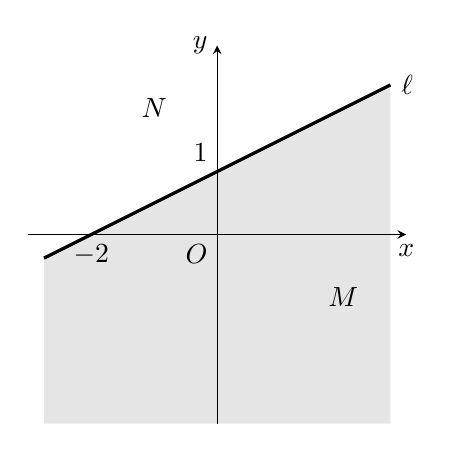
\begin{tikzpicture}[>=stealth, scale=.8]
    \fill[gray!20!white](-2.75,-.375)--(-2.75,-3)--(2.75,-3)--(2.75,2.375)--cycle;
  \draw[->](-3,0)--(3,0)node[below]{$x$};
  \draw[->](0,-3)--(0,3)node[left]{$y$};
\node[below left]{$O$};
\draw[domain=-2.75:2.75, very thick]plot(\x, 0.5*\x+1)node[right]{$\ell$};

\node at (0,1)[above left]{$1$};
\node at (-2,0)[below]{$-2$};

\node  at (2,-1){$M$};
\node at (-1,2){$N$};


\end{tikzpicture}    
\captionof{figure}{}
\end{minipage}


由此做出：
\begin{thm}
 {猜想1}
\begin{enumerate}
    \item 当$(x,y)\in M$时，恒有
\begin{equation}
   f(x,y)=x-2y+2>0 \tag{2}
\end{equation}
\item 当$(x,y)\in N$时，恒有
\begin{equation}
    f(x,y)=x-2y+2<0\tag{3}
\end{equation}
\end{enumerate}
\end{thm}

\begin{remark}
    这个猜想是合谐的. 若我们把$f(x,y)$看作是一个二元函数的话，上述猜想表明：
\begin{itemize}
  \item 在$M$上，函数$f(x,y)$的值处处恒正；
\item 在$\ell$上，函数$f(x,y)$的值处处恒为零；
\item 在$N$上，函数$f(x,y)$的值处处恒负.
\end{itemize}

（这里，函数、方程、不等式三个知识点又一次交汇在同一个问题之中）让我们来证明猜想1．
\end{remark}

\noindent
\begin{minipage}{.52\textwidth}\CTEXindent
\begin{proof}
任取$P_1(x_1,y_1)\in M$（图2.28），过点$P_1$作$P_1Q\bot x$轴交$\ell$于$Q(x_1,y_0)$, 于是$f(x_1,y_0)=x_1-2y_0+2=0$.

$\because\quad y_1<y_0$

$\therefore\quad 2y_1<2y_0  \Rightarrow -2y_1>-2y_0$

由此，
\[\begin{split}
    f(x_1,y_1)&=x_1-2y_1+2\\
    &>x_1-2y_0+2=0
\end{split} \]

$\therefore\quad $(2)成立，同理(3)也成立.
\end{proof}
\end{minipage}\hfill
\begin{minipage}{.45\textwidth}
    \centering
\begin{tikzpicture}[>=stealth, scale=.9]
  \draw[->](-2.5,0)--(3,0)node[below]{$x$};
  \draw[->](0,-1.5)--(0,3.5)node[left]{$y$};
\node[below left]{$O$};
\draw[domain=-2.5:2.75, very thick]plot(\x, 0.5*\x+1)node[right]{$\ell$};
\node at (2,2)[below right]{$Q(x_1,y_0)$};
\node at (2,.7)[right]{$P_1(x_1,y_1)$};

\tkzDefPoints{2/2/Q, 2/.7/P}
\tkzDrawPoints(P,Q)
\draw[dashed](P)--(Q);
\end{tikzpicture}    
\captionof{figure}{}
\end{minipage}


至此，我们证明了$M$（或$N$）上的所有的点的坐标都满足(2)（或(3)），也就是说，$M$（或$N$）上的所有的点坐标都是(2)（或(3)）的解. 问题引向深入，我们自然会从反面提出一个新问题：

\begin{thm}
    {猜想2} 不等式(2)的每一个解对应的点是否都在$M$上呢？
\end{thm}

\begin{remark}
     这个问题连同猜想1的解决将使$M$上的点集与不等式(2)的解集之间建立起一一对应的关系，从而使(2)能够成为区域$M$的代数形式. 所以，提出这两个猜想在理论上是很有价值的！
\end{remark}

让我们以图2.28为线索，证明猜想2．

\begin{proof}
设$(x',y')$是(2)的任一个解.则
\begin{equation}
    x'-2y'+2>0 \tag{3}
\end{equation}
在$\ell$上取点$(x',y_0')$，则
\begin{equation}
    x'-2y'+2=0 \tag{4}
\end{equation}
$(3)-(4)$，得$y'_0-y'>0 \quad\Rightarrow\quad y'<y'_0 \quad\Rightarrow \quad (x',y')\in M$

完全同样地，不等式(3)的每一个解对应的点也都在区域$N$上.
\end{proof}

我们把上述两个猜想联系起来可以看出：区域$M$与不等式(2)有非常密切的关系（这种关系同曲线与方程的关系十分类似！），抽象这种关系得到

\begin{thm}{区域与不等式的定义}
    对于平面上的点集$G$和不等式$f(x,y)>0$，若：
\begin{enumerate}
    \item $G$上每个点的坐标都是不等式的解；
    \item 不等式的每个实数解对应的点都在$G$上，称点集\textbf{$G$为$f(x,y)>0$的区域}，称\textbf{$f(x,y)>0$为区域$G$的不等式}.
\end{enumerate}
\end{thm}

至此，可以把上面的探索写成：

\begin{thm}
{结论} 直线$\ell$把全平面划分成两个区域和一条共同的边界线$\ell$，它们分别表示成：
$x-2y+2>0$, $x-2y+2<0$和$x-2y+2=0$.    
\end{thm}

推广这一结论，可得

\begin{thm}
    {定理} 直线$\ell:\; ax+by+c=0$把全平面分解成两个区域和一条共同的边界线，它们分别表示成
$ax+by+c>0$, $ax+by+c<0$和$ax+by+c=0$.
\end{thm}

这个定理的价值在于：它刻画了以直线为边界的平面区域与二元一次不等式之间的对应关系，奠定了用不等式研究平面区域的基础（定理的证明作为选作题）.

\begin{example}
    画出$x+2y-4<0$表示的区域.
\end{example}

\noindent
\begin{minipage}{.47\textwidth}
\CTEXindent
\begin{solution}
    先画出边界线（图2.29）

$\ell:\; x+2y-4=0$，再以$O'(0,1)$点的坐标代入$x+2y-4$得
\[x+2y-4=-4<0\]

$\therefore\quad O(0,0)$是$x+2y-4<0$的一个解.

由此原点所在的半平面区域就是$x+2y-4<0$的区域.
\end{solution}

\end{minipage}\hfill
\begin{minipage}{.47\textwidth}
    \centering
\begin{tikzpicture}[>=stealth, scale=.7]
  \draw[->](-2,0)--(6,0)node[below]{$x$};
  \draw[->](0,-2)--(0,4)node[left]{$y$};
\node[below left]{$O$};
\draw[domain=5:-1.75, very thick]plot(\x, 2-0.5*\x)node[above]{$\ell$};
\foreach \x in {2,4}
{
    \draw(\x,0)node[below]{$\x$}--(\x,.1);
}
\node at (0,2)[below left]{2};


\end{tikzpicture}    
\captionof{figure}{}
\end{minipage}

\begin{example}
    解不等式组
\[\begin{cases}
    x-2y+1<0 & (1)\\
    x+y-5<0 & (2)\\
    2x-y-1>0 & (3)\\
\end{cases}\]
\end{example}

\begin{analyze}
因为每个不等式各表示一个区域，所以解不等式组从几何上看就是去找各个不等式所确定的区域的\textbf{公共区域$G$}.
\end{analyze}

\begin{solution}
在平面上先作出直线（图2.30）:

\noindent
\begin{minipage}{.5\textwidth}
\[\begin{split}
    x-2y+1<0 &\qquad (\ell_1)\\
    x+y-5<0 & \qquad (\ell_2)\\
    2x-y-1>0 & \qquad (\ell_3)\\
\end{split}\]
\begin{itemize}
    \item 区域(1)在$\ell_1$的上方；
    \item 区域(2)在$\ell_2$的下方；
    \item 区域(3)在$\ell_3$的下方．
\end{itemize}

$\therefore\quad$区域(1)、(2)、(3)的公共区域是以$A(1,1)$、$B(3,2)$、$C(2,3)$为顶点的三角形区域$G$．$G$上的每一个点的坐标都是原不等式组的解.
\end{minipage}\hfill
\begin{minipage}{.47\textwidth}
    \centering
\begin{tikzpicture}[>=stealth]
  \draw[->](-1,0)--(4.5,0)node[below]{$x$};
  \draw[->](0,-1)--(0,4.5)node[left]{$y$};
\node[below left]{$O$};
\tkzDefPoints{1/1/A, 3/2/B, 2/3/C}
\draw[pattern=north east lines](A)--(B)--(C)--cycle;
\draw[domain=-.7:4 , very thick]plot(\x, 0.5+0.5*\x)node[above]{$\ell_1$};
\draw[domain=1:4 , very thick]plot(\x, 5-\x)node[below]{$\ell_2$};
\draw[domain=0.25:2.5 , very thick]plot(\x, 2*\x-1)node[above]{$\ell_3$};
\node at (A) [below right]{$A(1,1)$};
\node at (B) [right=.2]{$B(3,2)$};
\node at (C) [right]{$C(2,3)$};
\node at (2.1,2.1)[fill=white]{$G$};
\end{tikzpicture}    
\captionof{figure}{}
\end{minipage}
\end{solution}

    
\section*{习题五}
\begin{center}
    \bfseries A
\end{center}
\begin{enumerate}
    \item 点$(500,333)$、$(-500,-334)$、$(1,0)$在直线$2x-3y=1$的同侧吗？
    \item 画出$|3x+2y+4|\le 8$表示的区域.
    \item 画出$\begin{cases}
        x-y-2<0 \\2x+3y-12>0
    \end{cases}$所表示的区域.
\end{enumerate}


\begin{center}
    \bfseries B
\end{center}

\begin{enumerate}\setcounter{enumi}{3}
    \item 用不等式组写出以$(1,2)$、$(4,3)$和$(3,5)$为顶点的三角形区域.
\end{enumerate}

\section{本章小结}

\subsection{直线的倾斜角和斜率}
\begin{enumerate}
    \item 倾斜角$\alpha\in[0,\pi)$
    \item 斜率$k\in\R$
\[k=\begin{cases}
    \tan\alpha, & \alpha\ne \frac{\pi}{2}\\[1.5ex]
    \text{不存在}, &\alpha=\frac{\pi}{2}
\end{cases},\qquad k=\begin{cases}
    \frac{y_2-y_1}{x_2-x_1}, & x_1\ne x_2\\[1.5ex]
    \text{不存在}, &x_1=x_{2}
\end{cases}\]

\item $ \alpha=\begin{cases}
   \arctan k ,& k\ge 0\\
   \arctan k+\pi ,& k< 0\\
   \frac{\pi}{2},&\text{$k$不存在}\\[1.5ex]
\end{cases}$
\end{enumerate}

\subsection{直线方程的五种形式}
\begin{enumerate}
\item 点斜式：$y-y_1=k(x-x_1)$;
\item 斜截式：$y=kx+b$;
\item 两点式：$\frac{y-y_1}{y_2-y_1}=\frac{x-x_1}{x_2-x_1}$;
\item 截距式：$\frac{x}{a}+\frac{y}{b}=1$;
\item 一般式：$Ax+By+C=0$（$A$、$B$不全为零）.
\end{enumerate}

\subsection{两条直线所成的角}
\begin{enumerate}
    \item 到角的定义；
    \item 到角公式
\[\tan\theta_{1-2}=\frac{k_2-k_1}{1+k_2k_1}\]
应注意：当$k_1$、$k_2$都存在且$\theta_{1-2}\ne \frac{\pi}{2}$时才能使用这个公式；当$k_1$、$k_2$中至少有一个不存在时，应画出直线的草图，直观地分析问题.
\item 两条直线所成的角（夹角）的定义及夹角公式
\[\tan\theta=\left|\frac{k_2-k_1}{1+k_2k_1}\right|\]
\end{enumerate}

\subsection{两条直线平行或垂直的条件}
\begin{enumerate}
    \item 当$k_1$、$k_2$都存在时：
\begin{enumerate}[(1)]
    \item $\ell_1\parallel \ell_2\quad \text{（或$\ell_1$、$\ell_2$重合）} \Longleftrightarrow k_1=k_2$\hfill(1)
\item $\ell_1\bot \ell_2  \Longleftrightarrow k_1k_2=-1$\hfill(2)
\end{enumerate}
\item 当$k_1,k_2$中至少有一个不存在时，应画草图分析问题.
\item (1)(2)还可以用$\ell_1$、$\ell_2$方程$a_1x+b_1y+c_1=0$和$a_2x+b_2y+c_2=0$的系数表示出来.
\[\begin{split}
    \ell_1\parallel \ell_2 &\Longleftrightarrow \frac{a_1}{a_2}=\frac{b_1}{b_2}\ne \frac{c_1}{c_2}\\
    \text{$\ell_1$、$\ell_2$重合} &\Longleftrightarrow \frac{a_1}{a_2}=\frac{b_1}{b_2}= \frac{c_1}{c_2}
\end{split}\]
\begin{align}
    \therefore\quad \text{$\ell_1$、$\ell_2$平行（或重合）} &\Longleftrightarrow  a_1b_2-a_2b_1=0 \tag{1}\\
    \ell_1\bot \ell_2  &\Longleftrightarrow a_1a_2+b_1b_2=0\tag{2}
\end{align}

应注意，即使$k_1$、$k_2$不存在时，(3)、(4)也是成立的.

例如，当$k_1$不存在时，$b_1=0$, $a_1\ne 0$：

若$\ell_1$、$\ell_2$平行（或重合）则$\ell_2\parallel y$轴$\Rightarrow b_2=0$
    
    $\therefore\quad a_1b_2=a_2b_1=0$

若$a_1b_2-a_2b_1=0$，由$b_1=0,\; a_1\ne 0\Rightarrow b_2=0$
    
$\therefore\quad \ell_2\parallel y$轴$\Rightarrow \ell_1\parallel \ell_2$，或$\ell_1$、$\ell_2$重合.

$\therefore\quad \ell_1$、$\ell_2$平行（或重合）$\Longleftrightarrow a_1b_2-a_2b_1=0$.
\end{enumerate}

\subsection{两条直线的交点}
\begin{center}
\begin{tikzpicture}[>=stealth]
\node(A)[draw, rectangle] at (0,0)[text width=2cm, align=center]{$\ell_1$、$\ell_2$的\\交点问题};
\node(B) at (9,0)[left]{讨论$\begin{cases}
    a_1x+b_1y+c_1=0\\a_2x+b_2y+c_2=0
\end{cases}$的解集问题：};
\draw[<->, very thick](A)--(B);
\end{tikzpicture}
\end{center}
\begin{enumerate}
    \item $a_1b_2-a_2b_1\ne 0$时，$\ell_1$、$\ell_2$相交于一点；
    \item $a_1b_2-a_2b_1=0$时，$\ell_1$、$\ell_2$平行或重合.
\end{enumerate}

\subsection{点$P_0(x_0,y_0)$到$\ell:\; ax+by+c=0$的距离，平行直线$\ell_1$、$\ell_2$的距离}
\begin{enumerate}
    \item 点到直线距离的定义，
    \item 距离公式
\[\begin{split}
 \ell_1:\;   ax+by+c_1&=0\\ 
 \ell_2:\;   ax+by+c_2&=0\\ 
\end{split}\]
\end{enumerate}

\begin{center}
    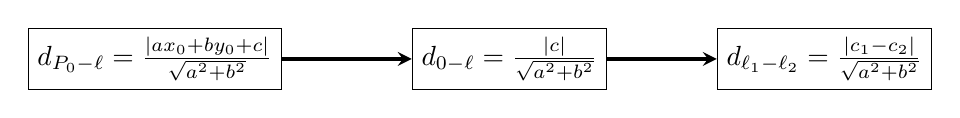
\begin{tikzpicture}[>=stealth]
        \node(A)[draw, rectangle] at (0,0){$d_{P_0-\ell}=\frac{|ax_0+by_0+c|}{\sqrt{a^2+b^2}}$};
        \node(A1)[draw, rectangle] at (4.5,0){$d_{0-\ell}=\frac{|c|}{\sqrt{a^2+b^2}}$};
        \node(A2)[draw, rectangle] at (8.5,0){$d_{\ell_1-\ell_2}=\frac{|c_1-c_2|}{\sqrt{a^2+b^2}}$};
\draw[->, very thick](A)--(A1);
\draw[->, very thick](A1)--(A2);
    \end{tikzpicture}
\end{center}

\subsection{关于直线的对称点}
\begin{center}
\begin{tikzpicture}[>=stealth]
    \node(A)[draw, rectangle] at (0,0)[text width =3cm, align=center]{点关于直线$\ell$的\\对称点的定义};
    \node(A1)[draw, rectangle] at (5,0)[text width =4cm, align=center]{点关于一些特殊直线的\\对
    称点的求法（要熟练）};
    \draw[->, very thick](A)--(A1);
\node(B)[draw, rectangle] at (2,-3.5)[text width =7.5cm]{点$P$关于直线$\ell:\; ax+by+c=0\; (ab\ne 0)$的\\
对称点$P'$的求法：\\
依定义有\\
$\begin{cases}
    \ell\bot PP'\Leftrightarrow k_{\ell}\cdot k_{PP'}=-1&\rm (A)\\
    \text{$\ell$平分$PP'$}\Leftrightarrow \text{$PP'$的中点在$\ell$上}&\rm (B)
\end{cases}$\\
把(A)、(B)转化成代数形式即可.};
\draw[->, very thick](A)--(0,-1.7);
\node(C)[draw, rectangle] at (2,-7)[text width =7cm]{解光线经过镜面（直线）的反射问题：\\
依据：光的最短路径原理.\\
数学工具：点关于直线的对称点的方法.};
\draw[->, very thick](B)--(C);



















\end{tikzpicture}
\end{center}

\subsection{直线系}

\begin{enumerate}
    \item 与$ax+by+c=0$平行的直线系是
 \[   ax+by+m=0\quad (m\ne c)\]
    \item 与$ax+by+c=0$垂直的直线是
   \[ bx-ay+n=0\]
    \item 过$(x_0,y_0)$的直线系是$x=x_0$或$y-y_0=k(x-x_0)$，其中$k\in\R$.
    \item 过$\ell_1:\; a_1x+b_1y+c_1=0$和$\ell_2:\; a_2x+b_2y+c_2=0$交点的直线系（不含直线$\ell_2$）是
\[    a_1x+b_1y+c_1+\lambda (a_2x+b_2y+c_2)=0\] 
其中参数$\lambda\in\R$
\end{enumerate}

\subsection{以$\ell:\; ax+by+c=0$为边界的平面区域}
见2.10节








































































































\section*{复习题一}
\begin{center}
    \bfseries A
\end{center}

\begin{enumerate}
\item 用坐标法证明：
\begin{enumerate}[(1)]
\item 在直角三角形中，斜边中点与三个顶点距离相等，其逆命题也真；
\item 在正方形$ABCD$中，$E$是$BC$上一点，若$DE=AB+EB$，求证：$BE=\frac{1}{4}AB$,
\item 正三角形内任一点到三边距离之和为一定值．
\end{enumerate}

\item 一条直线平行于直线$3x-4y-20=0$，并且和它相距3个单位，求这条直线的方程.
\item 求垂直于直线$3x+4y=7$，且分别适合下列条件的直线的方程：
\begin{enumerate}[(1)]
\item 与两坐标轴围成的三角形的周长为10；
\item 与两坐标轴围成的三角形的面积为直线$3x+4y=7$与两坐标轴围成的三角形面积的2倍；
\item 与原点的距离为4．
\end{enumerate}

\item 直线$\ell_1:\; x+3=0$，到$\ell_2:\; x-y-2=0$的角$\theta=\blank$，$\ell_1$与$\ell_2$的夹角$\alpha=\blank$.
\item （选择题）直线$(2m^2+m-3)x+(m^2-m)y=2m$与直线$x-y=1$平行，则$m$的值是（\qquad ）.
\begin{multicols}{4}
\begin{enumerate}[(A)]
    \item 1
    \item $-1$
    \item $\pm 1$
    \item 不存在
\end{enumerate}
\end{multicols}

\item （选择题）直线$ax+by+c=0\; (ab>0)$的倾斜角是（\qquad）.
\begin{multicols}{2}
\begin{enumerate}[(A)]
    \item $\arctan\frac{a}{b}$
    \item $\arctan\left(-\frac{a}{b}\right)$
    \item $\pi-\arctan\frac{a}{b}$
    \item $\pi+\arctan\frac{a}{b}$
\end{enumerate}
\end{multicols}
\end{enumerate}


\begin{center}
    \bfseries B
\end{center}

\begin{enumerate}\setcounter{enumi}{6}
    \item  若$A(x_1,y_1)$、$B(x_2,y_2)$是斜率为$k$的直线$\ell$上的两个点，试证明：
\begin{multicols}{2}
\begin{enumerate}[(1)] 
    \item $|AB|=|x_1-x_2|\cdot \sqrt{1+k^2}$
    \item $|AB|=|y_1-y_2|\cdot \sqrt{1+\frac{1}{k^2}}$
\end{enumerate}
\end{multicols}

    \item  直线$\ell$过点$(1,0)$，且被两平行线$3x+y-6=0$和$3x+y+3=0$所截得的线段长为3，求$\ell$的方程．
    \item $\triangle ABC$三顶点是$A(0,0)$、$B(8,0)$、$C(7,6)$;
\begin{enumerate}[(1)]
    \item 求重心$M$、垂心$H$、外心$G$的坐标；
    \item 证明$M$、$H$、$G$共线．
\end{enumerate}

    \item \begin{enumerate}[(1)]
        \item 已知直线$\ell$过原点且倾斜角为$\alpha\; \left(\alpha\ne \frac{\pi}{2}\right)$，$A'$是点
    $A(a,b)$关于$x$轴的对称点，试求$A'$关于$\ell$的对称点B的坐标；
    \item 已知$A(-2,2)$、$B(-3,-1)$和直线$\ell:\; y=2x-1$, 试在$\ell$上求一点$P$，使$|PA|+|PB|$为最小.
    \end{enumerate}

    \item  设点$P_0(x_0,y_0)$在直线$ax+by+c=0$上，求证：这条直线的方程可以写成$a(x-x_0)+b(y-y_0)=0$.
\item 已知$\ell_1:\; 2x-2y-3=0$，$\ell_2:\; 3x-5y+1=0$，$\ell_3:\; ax+y+b=0$
\begin{enumerate}[(1)]
    \item 求三条直线共点（相交于一点）的充要条件；
    \item 当三直线共点时，确定$a$，$b$的值，使$\ell_2$、$\ell_3$关于$\ell_1$对称.
\end{enumerate}

\item 已知$\triangle ABC$中，$A(3,-1)$, $\angle ABC$的平分线所在方程为$x-4y+10=0$，$AB$边上的中线方程为$6x+10y-59=0$，求点$B$的坐标和$BC$边所在直线的方程.
\end{enumerate}

\begin{center}
    \bfseries C
\end{center}

\begin{enumerate}\setcounter{enumi}{13}
 \item 已知直线$\ell:\; 4x-y=0$和$P(6,4)$. 过点$P$引一条直线$\ell'$，使$\ell$、$\ell'$、$x$轴三者在第一象限内围成的三角形面积最小，求$\ell'$的方程.

 \item 过点$P(2,1)$作直线$\ell$，分别交$x$、$y$轴正半轴于$A$、$B$两点，求分别满足下列条件时$\ell$的方程：
 \begin{enumerate}[(1)]
 \item 使得$\triangle ABO$的面积最小（$O$为原点）；
 \item 使得在两轴上的截距之和为6；
 \item 使得$|PA|\cdot |PB|$的值最小.
 \end{enumerate}

 \item 要使直线$y=kx+b$与直线$2x-y-4=0$的夹角为$45^{\circ}$，
 且交点在第一象限，试确定$k$的值和相应的$b$的取值范围.
\end{enumerate}